\documentclass[a4paper,12pt]{report}
\usepackage[utf8]{inputenc}
\usepackage{graphicx}
\usepackage{amsmath}
\usepackage{float}
\usepackage{biblatex}
\usepackage{csquotes}
\usepackage{centernot}
\usepackage{amssymb}
\usepackage{mathtools}
\usepackage{titling}
\usepackage{textcomp}
\usepackage{pgfplots}
\usepackage{pdfpages}
\usepackage{tcolorbox}
\usepackage{fontawesome}
\usepackage{xfrac}
\usepackage{xcolor}
\usepackage{pagecolor}

\usepackage{hyperref}




\newcommand{\suc}{X_i, ... ,X_n}
\newcommand{\somsuc}{X_i + ... + X_n}
\newcommand{\va}{X_i}
\newcommand{\disc}{P_{X_i}(x)=p(x)}
\newcommand{\ac}{f_{X_i}(x)=f(x)}
\newcommand{\ind}{\noindent}
\newcommand{\n}{\newline}
\newcommand{\mc}{\overline{{X}_N}}
\newcommand{\sn}{S_{n}^{2}}
\newcommand{\xn}{X^2(n)}
\newcommand{\dsum}{\displaystyle\sum}
\newcommand{\std}{\dfrac{\somsuc - E[X]}{\sqrt{Var[X]}}}
\newcommand{\pP}{\text{I\kern-0.15em P}}
\newcommand{\chiqm}{\chi^2(n)}
\newcommand{\chiqmn}{\chi^2(n-1)}

\usepackage[italian]{babel}
\pgfplotsset{compat=1.18}

\begin{document}

\begin{titlepage}
    \begin{center}
        \vspace*{1cm}
            
        \Huge
        \textbf{Probabilità e Statistica per l'Informatica}
            
        \vspace{0.5cm}
        \LARGE
        Ver 1.1
            
        \vspace{1.5cm}
            
        \textbf{Falbo Andrea}
            
        \vfill
            
        A.A 2022/2023 \\
        \faGithub{LilQuacky}
            
        \vspace{0.8cm}
            
        
\includegraphics[width=0.4\textwidth]{Foto/duck-png-20143.png}
            
    \end{center}
\end{titlepage}

\tableofcontents
\newpage
\pagecolor{lightgray}
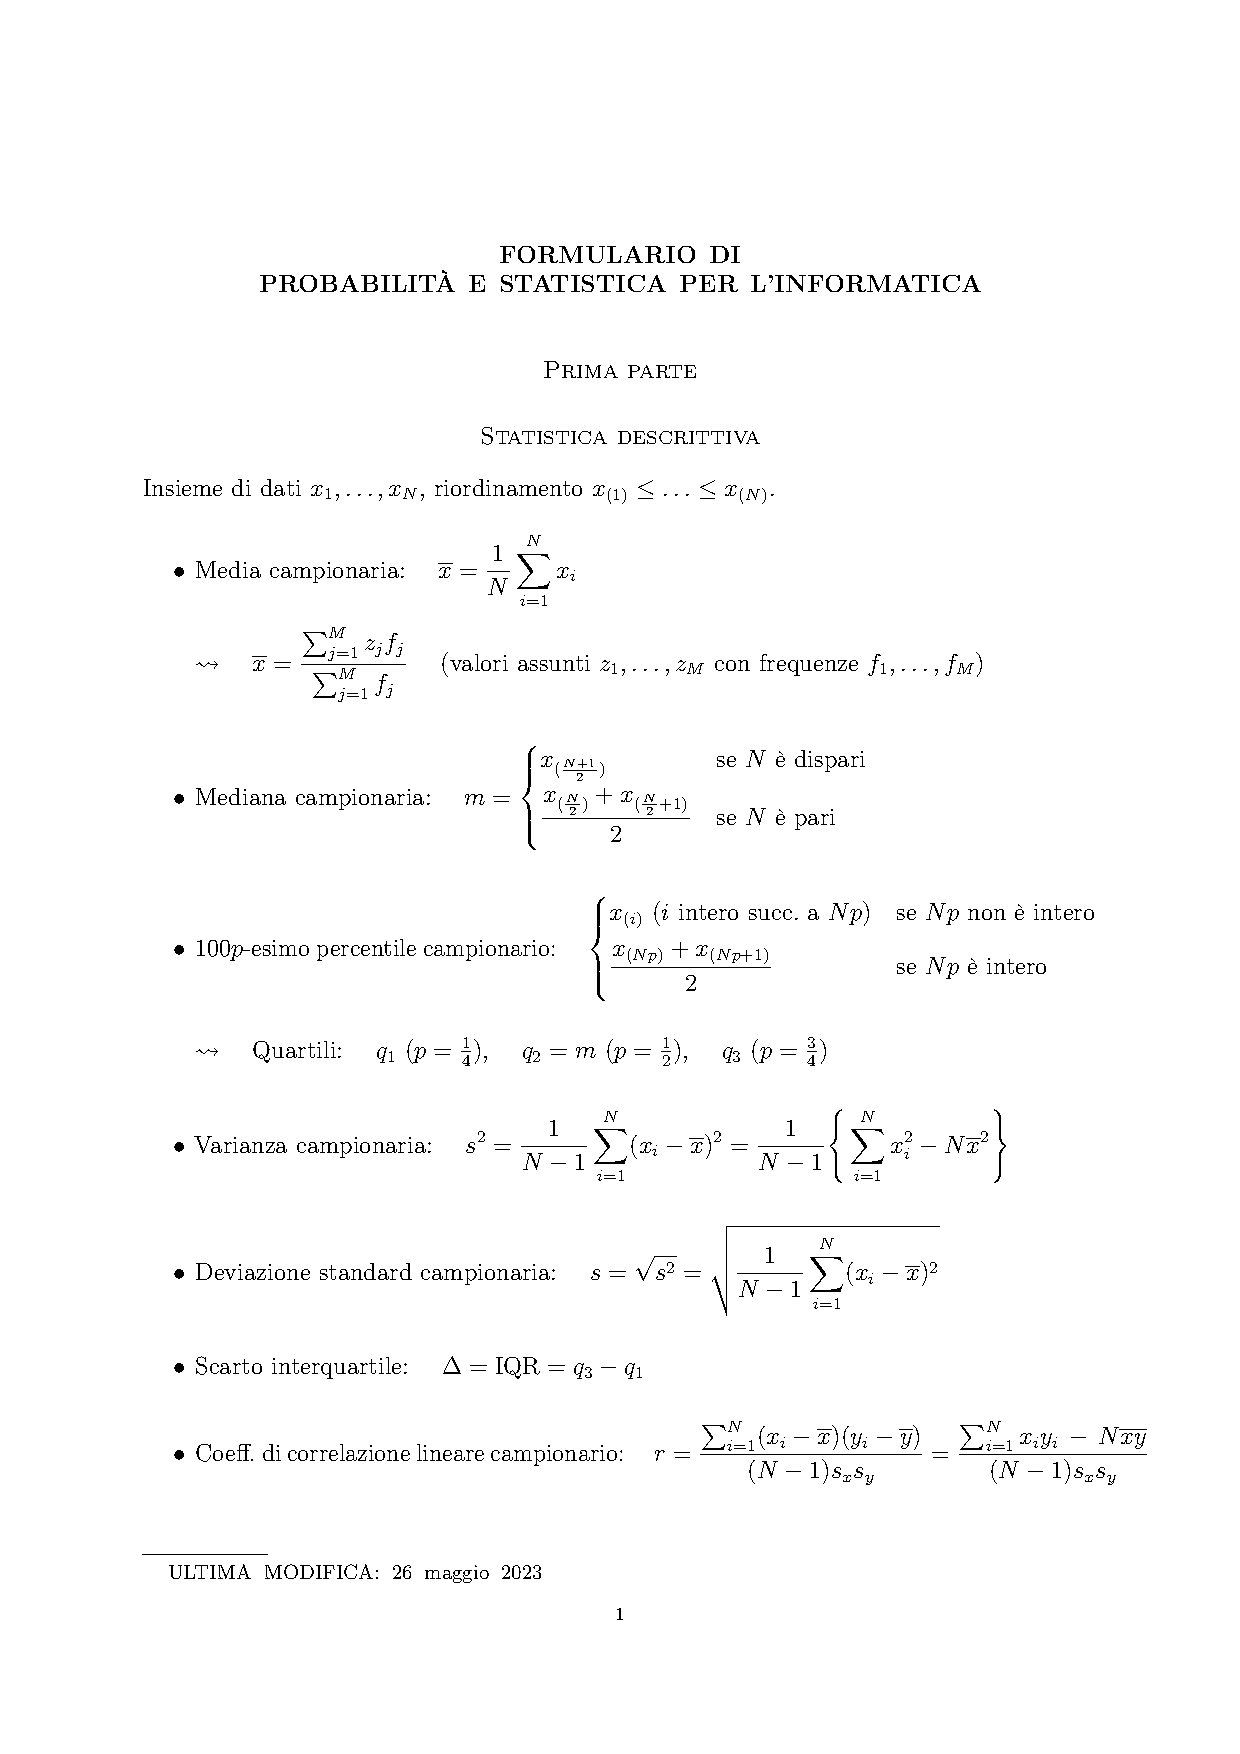
\includepdf[pages=-]{pdf/formulario-PSI.pdf}
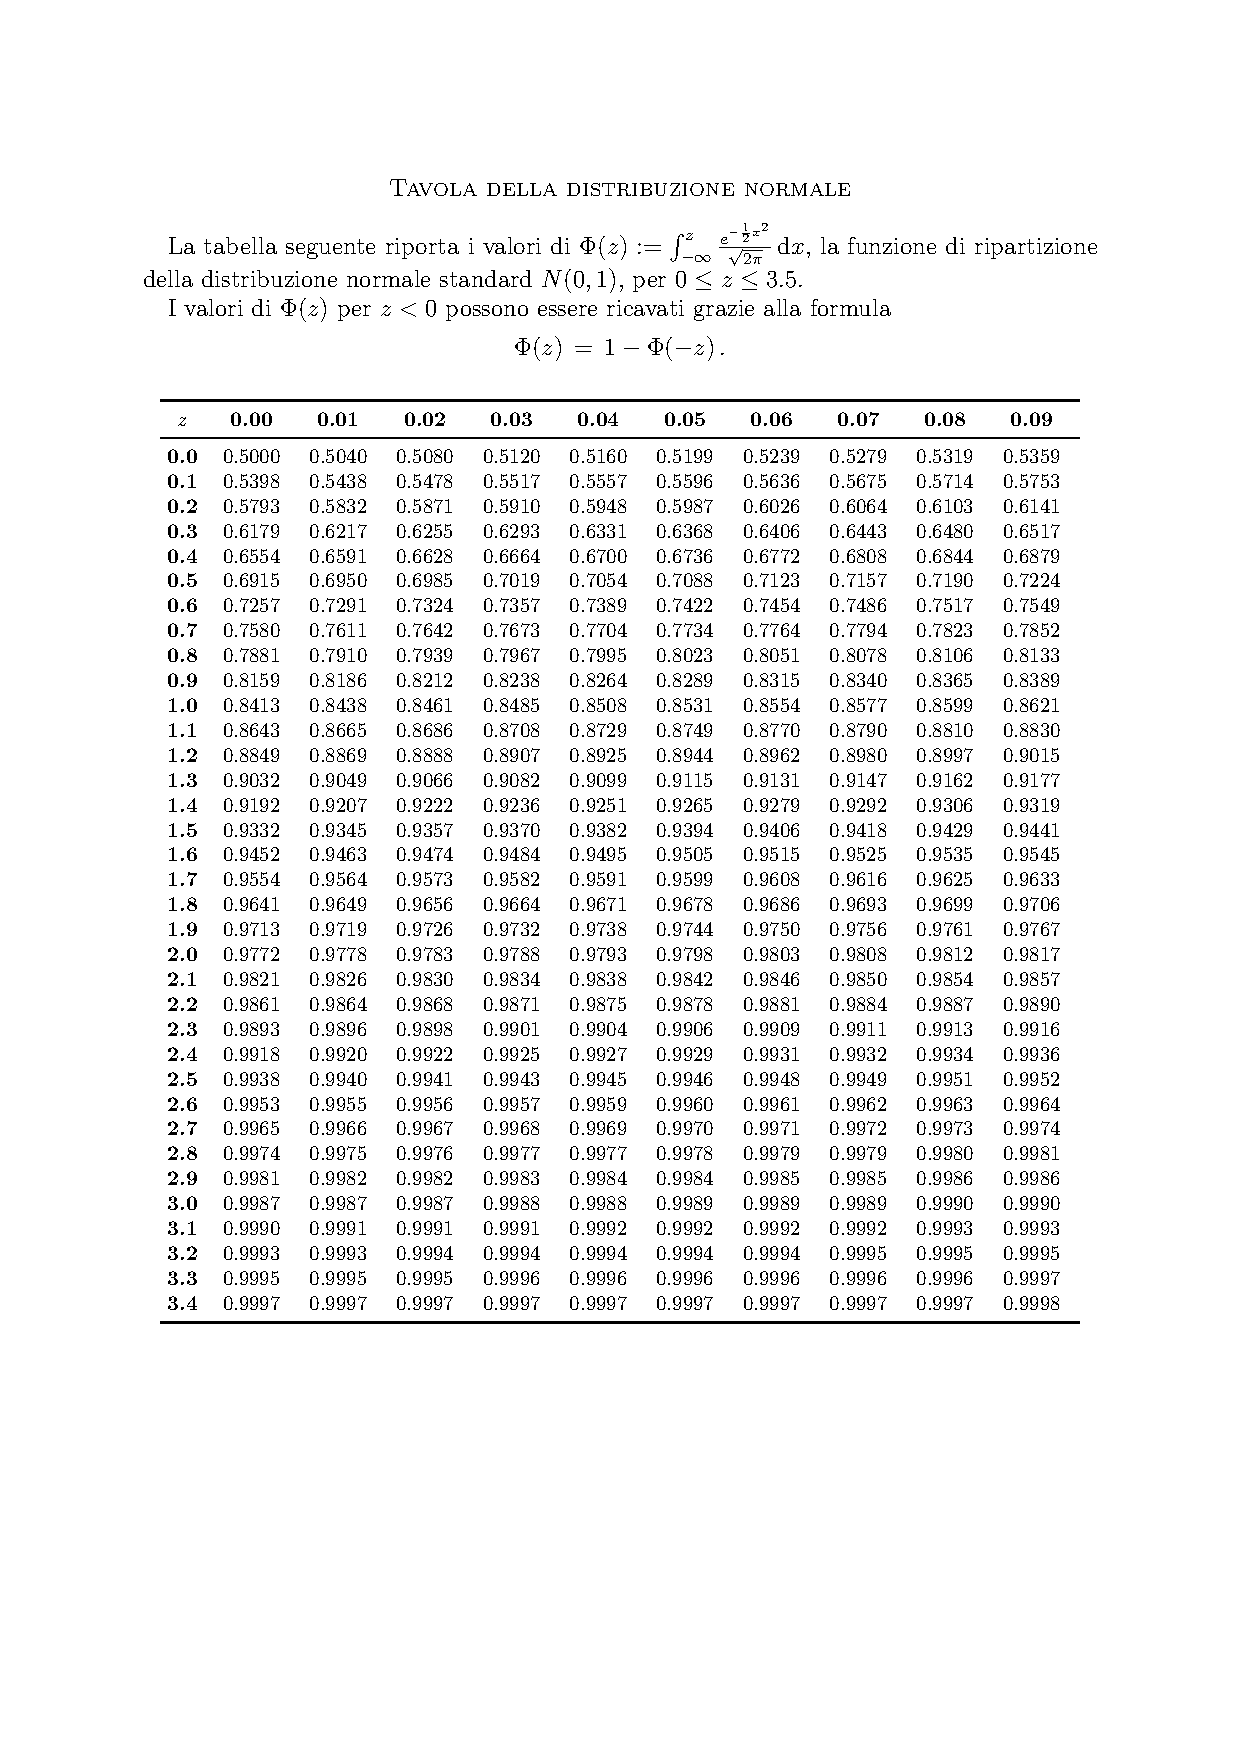
\includepdf[pages=-]{pdf/tavole-insieme.pdf}
\nopagecolor
\renewcommand{\labelitemi}{\textsc{\labelitemiv}}

\chapter[Statistica Descrittiva]{Statistica Descrittiva}

\section{Introduzione}

\subsubsection{Statistica Descrittiva, Statistica Inferenziale e Probabilità}

La statistica è l'arte di imparare dai dati. Possiamo suddividerla in:
\begin{itemize}
    \item \textbf{Statistica Descrittiva}: \textit{Descrive} e riassume i dati
    \item \textbf{Statistica Inferenziale}: \textit{Trae} conclusioni dai dati
\end{itemize}
Per poter trarre conclusioni dai dati, bisogna tenere conto del ruolo che gioca il caso. Definiamo quindi la \textbf{probabilità} come la descrizione matematica di eventi \textit{casuali}.

\section{Descrivere i dati}

\subsection{Frequenze, Istogrammi, Classi}

\subsubsection{Frequenza Assoluta e Relativa}

Misuriamo una certa variabile in un campione, ottenendo un insieme di dati. Se i dati non sono distinti, ovvero \textit{abbiamo ripetizioni}, possiamo riassumerli in una \textbf{tabella delle frequenze}. Possiamo definire dunque:

\begin{itemize}
    \item \textbf{Frequenza Assoluta $f_i$ }:= numero di volte in cui i compare nel campione di dati.
    \item \textbf{Frequenza Relativa $p_i$ }:= $\sfrac{f_i}{N}$ = numero di volte in cui compare i rispetto al totale.  
\end{itemize}

\begin{tcolorbox}
    \textbf{Esempio}: Marta intervista i suoi N = 20 compagni di classe e chiede la squadra di calcio preferita, ottenendo le risposte: \newline \textit{Juve, Milan, Inter, Atalanta, Juve, Milan, Nessuna, Nessuna, Inter, Milan, Juve, Nessuna, Atalanta, Juve, Nessuna, Milan, Inter, Milan, Nessuna, Nessuna}. \newline
    
    \begin{tabular}{ |p{3.5cm}|p{3.5cm}|p{3.5cm}|  }
        \hline
        \multicolumn{3}{|c|}{Squadre di Calcio} \\
        \hline
        Valori & Frequenze assolute & Frequenze relative \\
        \hline
        Juve & 4 & 4/20 = 0.20 \\
        Milan & 5 & 5/20 = 0.25 \\
        Inter & 3 & 3/20 = 0.15 \\
        Nessuna & 6 & 6/20 = 0.30 \\
        Atalanta & 2 & 2/20 = 0.10 \\
        \hline
    \end{tabular}
\end{tcolorbox}

\subsubsection{Istogramma}

É utile rappresentare le frequenze mediante un grafico a barre detto \textbf{istogramma}. \newline

\begin{figure}[htbp]
    \centering
    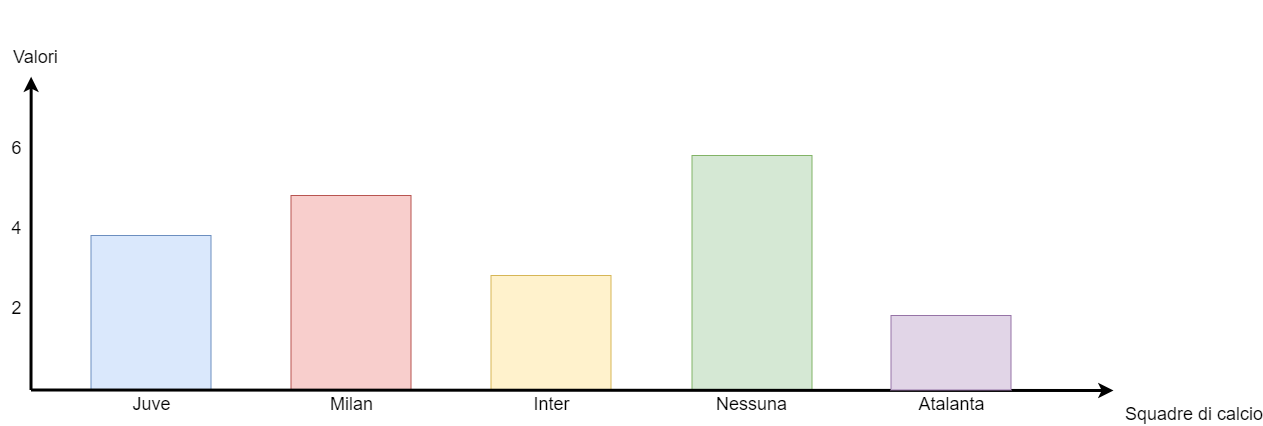
\includegraphics[scale=.4]{Foto/barchart.png}
    \color{gray}
    \caption{Istogramma sulle frequenze assolute delle squadre di calcio} 
\end{figure}

\newpage
\subsubsection{Classi}

Può capitare di avere insiemi di dati che assumono un numero elevato di valori distinti. In tal caso conviene \textit{suddividere} i valori assunti in intervalli detti \textbf{classi}. \newline

\begin{tcolorbox}
\textbf{Esempio}: Vengono misurati i livelli di colesterolo nel sangue di un insieme di N = 40 individui: 
\begin{center}
    213 174 193 796 220 183 194 200 192 200  200 199 178 183 188 193 187 181 193 205 196 211 202 213 216 206 195 191 171 194 184 191 221 212 221 204 204 191 183 227
\end{center}
Molti valori sono distinti e dunque hanno $f_i = 1$. Scegliamo le classi: 
\begin{center}
    ${[170,180) \quad [180,190) \quad [190,200) \quad [200,210) \quad [210,220) \quad [220,230)}$
\end{center}

\begin{tabular}{ |p{3.5cm}|p{3.5cm}|p{3.5cm}|  }
    \hline
    \multicolumn{3}{|c|}{Livelli di colesterolo} \\
    \hline
    Valori & Frequenze assolute & Frequenze relative \\
    \hline
    $[170,180)$ & 3 & 3/40 = 7.5 \\
    $[180,190)$ & 7 & 7/40 = 17.5 \\
    $[190,200)$ & 13 & 13/40 = 32.5 \\
    $[200,210)$ & 8 & 8/40 = 20 \\
    $[210,220)$ & 5 & 5/40 = 12.5 \\
    $[220,230)$ & 4 & 4/40 = 10 \\
    \hline
\end{tabular}
\end{tcolorbox}

\newpage
\subsection{Dati Bivariati}


I \textbf{dati bivariati} ci permettono di mostrare \textit{due variabili} per ogni singolo elemento dell'insieme. Per un elemento i, indichiamo con $x_i$ la prima variabile e con $y_i$ la seconda.

\subsubsection{Diagramma Di Dispersione} 

Un \textbf{diagramma di dispersione} rappresenta i punti ($x_i$, $y_i$), in modo da evidenziare una possibile \textit{correlazione} tra i due valori.\newline

\begin{tcolorbox}
    \textbf{Esempio}: Rileviamo il numero di anni di scuola (prima variabile) e le pulsazioni a riposo (seconda variabile) in un campione di N=10 individui. I dati ($xi$ , $yi$) sono
    \begin{center}
        (12,73) (16,67) (13,74) (18,63) (19,73) (12,84) (18,60) (19,62) (12,76) (14,71)
    \end{center}
    \centering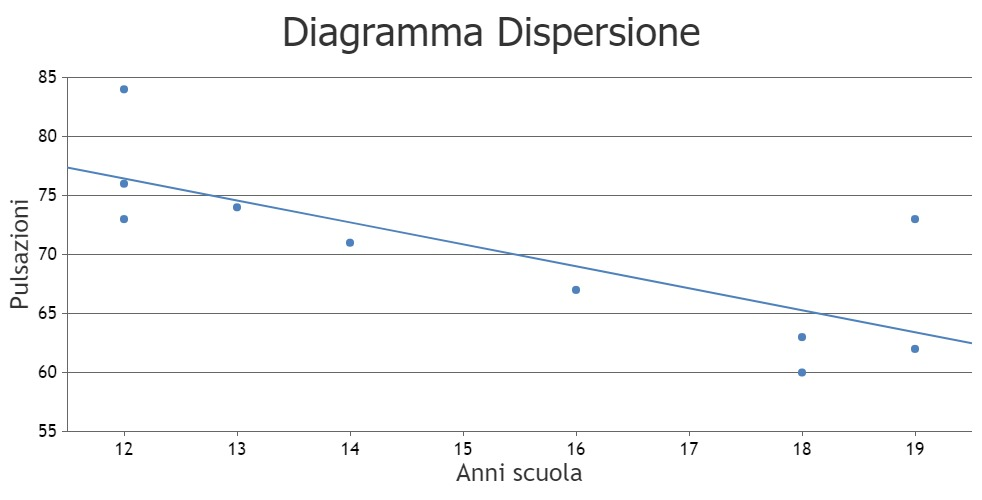
\includegraphics[scale=.3]{Foto/Chart.jpeg} \newline
    Possiamo evidenziare una correlazione negativa tra i due valori.

\end{tcolorbox}

\newpage
\section{Riassumere i dati}

Una \textbf{statistica} campionaria riassume l'insieme di dati mediante una quantità numerica.

\subsection{Indici di Posizione}

Un \textbf{indice di posizione} \textit{sintetizza la posizione} di una distribuzione sostituendo l'insieme dei dati con un unico valore tale da fornire una rappresentazione globale.

\subsubsection{Media Campionaria}

Per definire il valore medio dell'insieme dei dati, definiamo la \textbf{media campionaria} come $$ \overline{x} := \dfrac{x_1 + x_2 + \cdots + x_N}{N} = \dfrac{1}{N} \sum_{i=1}^n x_i $$

\noindent In generale, sapendo le frequenze assolute dei valori, possiamo scrivere la media campionaria come $$ \overline{x} = \dfrac{z_1 \cdot f_1 + z_2 \cdot f_2 + \cdots + z_M \cdot f_M}{N}$$ con $N= f_1 + f_2 + \cdots + f_M$, dove $z_i$ sono i valori e $f_i$ sono le frequenze assolute associate. \newline

\noindent \textbf{Osservazione}: La media è lineare: $\overline{y} = a \cdot \overline{x} + b$ 

\subsubsection{Mediana Campionaria}

Un'altra misura del centro dell'insieme dei dati è la \textbf{mediana campionaria}, ovvero quel valore che, ordinati i dati, si trova in \textit{posizione centrale}. In base al numero di dati, si calcola in due modi:

\begin{itemize}
    \item \textbf{N dispari}: la mediana è il dato di posto $\frac{N+1}{2}$ :  $$ m := x_{\left(\frac{N+1}{2}\right)} $$ 
    \item \textbf{N pari}: la mediana è la media aritmetica tra il dato di posto $\frac{N}{2}$ e quello di posto $\frac{N}{2} + 1$ :  $$ m := \frac{x_{\left(\frac{N}{2} \right)} + x_{\left(\frac{N}{2}+1\right)}}{2} $$
\end{itemize}

\subsubsection{Percentile Campionario}

Fissiamo un numero $ k \in [0, 100]$. Definiamo il \textbf{k-esimo percentile campionario} il valore t per cui:
\begin{itemize}
    \item almeno il $k\%$ dei dati è $\leq$ t
    \item almeno il $(100-k)\%$ dei dati è $\geq$ t
\end{itemize}

\subsubsection{Quartili}

I casi più importanti sono:
\begin{itemize}
    \item \textbf{Primo Quartile} $q_1$: $p = \dfrac{1}{4}$, $k=100p$
    \item \textbf{Secondo Quartile} $q_2$: $p = \dfrac{1}{2}$, $k=100p$
    \item \textbf{Terzo Quartile} $q_3$: $p = \dfrac{3}{4}$, $k=100p$
\end{itemize}

\noindent Come per la mediana, si calcola in due modi:
\begin{itemize}
    \item Se $N \cdot p$ non è intero, $t=x_{(i)}$ è il dato di posizione i definito come l'intero successivo a $N \cdot p$
    \item Se $N \cdot p$ è intero, $t= \dfrac{x_{(N \cdot p)} + x_{(N\cdot p+1)}}{2}$
\end{itemize}

\begin{tcolorbox}
    \textbf{Esempio}: Ai 1000 abitanti di un piccolo comune viene chiesto di esprimere un giudizio su un nuovo servizio comunale, usando una scala da 0 a 4. 251 persone hanno votato 0, 260 persone hanno votato 1, 80 persone hanno votato 2, 154 persone hyanno votato 3 mentre 255 persone hanno votato 4\newline
    Vogliamo calcolare i 3 indici di posizione: Media, Mediana, Quartili. \newline
    \begin{itemize}
        \item \textbf{Media}: $\overline{x} = \dfrac{0 \cdot 251 + 1 \cdot 260 + 2 \cdot 80 + 3 \cdot 154 + 4 \cdot 255}{1000}= 1,902 \simeq 1,9$
        \item \textbf{Mediana}: $m = \dfrac{x_{(500)} + x_{(501)}}{2} = \dfrac{1+1}{2}= 1$
        \item \textbf{Primo quartile}: $1000 \cdot \dfrac{1}{4} = 250 $, $q_1 = \dfrac{x_{(250)} + x_{(251)}}{2} = \dfrac{0+0}{2}=0$
        \item \textbf{Secondo quartile}: mediana = 1
        \item \textbf{Terzo quartile}: $ 1000 \cdot \dfrac{3}{4} = 750 $, $q_3 = \dfrac{x_{(750)} + x_{(751)}}{2} = \dfrac{4+4}{2}=4$
    \end{itemize}
\end{tcolorbox} 

\subsubsection{Box Plot}

Una rappresentazione grafica di mediana e quartili viene fornita dal \textbf{box plot}:
\begin{figure}[h!]
    \centering
    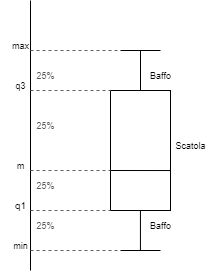
\includegraphics[scale=.6]{Foto/baba.png}
\end{figure}

\subsection{Indici di Dispersione}

Un \textbf{indice di dispersione} descrive la \textit{variabilità di distribuzione} quantitativa dei dati, ovvero quanto i valori presenti distano da un valore centrale.  

\subsubsection{Scarti}

Gli \textbf{scarti} sono la distanza di ogni singolo elemento dal valore medio. La somma di tutti gli scarti è nulla. $$w:= (x_i - \overline{x})$$ 

\subsubsection{Varianza Campionaria}

Considerando gli scarti elevati al quadrato e facendone una sorta di media, otteniamo la \textbf{varianza campionaria} come: $$ s^2 := \dfrac{1}{N-1} \sum_{i=1}^N(x_i - \overline{x})^2 $$ 

\subsubsection{Deviazione Standard}

Per ottenere una statistica omogenea ai dati, si definisce \textbf{deviazione standard} come: $$ s := \sqrt{s^2} = \sqrt{\dfrac{1}{N-1} \sum_{i=1}^N(x_i - \overline{x})^2}$$ 

\subsubsection{Scarto Interquartile}

Un altro indicatore di dispersione rispetto alla mediana m è lo \textbf{scarto interquartile}. Per costruzione, questo intervallo contiene almeno il 50\% dei dati. Il suo valore è: $$ IQR = \Delta := q_3 - q_1$$  \newline

\noindent \textbf{Osservazione}: La varianza e la deviazione standard non sono lineari. \newline 

%\noindent \textbf{Teorema}: L'intervallo attorno a $\overline{x}$ di ampiezza proporzionale a $s$: $$(\overline{x} - c \cdot s, \overline{x} + c \cdot s) \qquad c \geq 0$$ contiene una frazione di dati pari a: $$\alpha \geq 1 - \dfrac{1}{c^2} $$ Ad esempio, se c=2, avremo il 75\% dei dati nell'intorno, con c=3 avremo l'89\%.% 

\subsection{Correlazione}

Consideriamo un insieme di dati bivariati. Vogliamo quantificare la correlazione tra le due variabili x e y, ossia la \textit{tendenza} per cui a valori di x grandi corrispondo valori di y grandi o piccoli. Definiamo quindi il \textbf{coefficiente di correlazione lineare}: $$r =  \dfrac{ \sum_{i=1}^N (x_i-\overline{x})(y_i - \overline{y})}{(N-1)\cdot s_x \cdot s_y} \quad \text{oppure} \quad r =  \dfrac{ \sum_{i=1}^N x_i \cdot y_i - N \cdot \overline{x} \cdot \overline{y}}{(N-1)\cdot s_x \cdot s_y}$$  Il coefficiente di correlazione lineare può assumere valori $\in [-1, 1]$. Nello specifico diremo che:
\begin{itemize}
    \item $|r| \gtrsim 0,7$ avremo correlazione \textit{significativa}
    \item $|r| \lesssim 0,3$ avremo correlazione \textit{debole}.
\end{itemize} 

\begin{tcolorbox}
    \textbf{Esercizio Completo}: Prendiamo un campione di N = 10 elementi e assegnamo x = numero anni di scuola e y = pulsazioni. Otteniamo i seguenti valori 
    \begin{center}
        (12, 73) (16, 67) (13, 74) (18, 63) (19, 73) (12, 84) (18, 60) (19, 62) (12, 76) (14, 71)
    \end{center}
    Calcoliamo $\overline{x}, m, s^2, s, r$.
    \begin{itemize}
        \item $\overline{x} = \frac{12 + 16 + 13 + 18 + 19 + 19 + 12 + 18 + 19 + 12 + 14}{10} = 15,3$
        \item $s_{x}^2 = \frac{(12 + 16 + 13 + 18 + 19 + 19 + 12 + 18 + 19 + 12 + 14)^2 - 10 \cdot (15,3)^2}{9} \simeq 9,12$
        \item $s_x = \sqrt{s_{x}^2} \simeq 3,02 $
        \item $\overline{y} = \frac{73 + 67 + 74 + 63 + 73 + 84 + 60 + 62 + 76 + 71}{10} = 70,3$
        \item $s_{y}^2 = \frac{(73 + 67 + 74 + 63 + 73 + 84 + 60 + 62 + 76 + 71)^2 - 10 \cdot (70,3)^2}{9} \simeq 54,23$
        \item $s_y = \sqrt{s_{y}^2} \simeq 7,36 $
        \item $ \dsum_{i=1}^N x_i \cdot y_i = 12 \cdot 73 + 16 \cdot 67 + 13 \cdot 74 + \cdots + 14 \cdot 71 = 10603$
        \item $ r = \frac{10603 - 10 \cdot 15,3 \cdot 70,3}{9 \cdot 3,02 \cdot 7,36} \simeq -0,76$
    \end{itemize}
    Il valore di r conferma che x e y mostrano una significativa correlazione negativa
\end{tcolorbox} 




    
\renewcommand{\labelitemi}{\textsc{\labelitemiv}}

\chapter[Spazi di Probabilità]{Spazi di Probabilità}

\section{Introduzione}

Il \textbf{calcolo delle probabilità} è una teoria matematica che permette di descrivere gli \textit{esperimenti aleatori}, ovvero fenomeni il cui esito non è prevedibile con certezza a priori.

\section{Assiomi della Probabilità}

\subsubsection{Spazio Campionario, Evento, Probabilità}

La descrizione matematica di esperimento aleatorio si descrive in 3 passi:
\begin{enumerate}
    \item \textbf{Spazio Campionario}: Insieme $\Omega$ che contiene tutti i possibili esiti dell'esperimento. 
    \item \textbf{Eventi}: Affermazioni sull'esito dell'esperimento aleatorio. $A \subseteq \Omega$. 
    \item \textbf{Probabilità}: Funzione P che associa a ogni evento $A \subseteq \Omega$ un valore $\in [0, 1]$ che soddisfa opportune proprietà. Ci sono almeno due interpretazioni su che cos'è P(A):
        \begin{itemize}
            \item \textbf{Soggettivista}: P(A) = prezzo equo di una scommessa che paga 1 se si verifica A, altrimenti 0.
            \item \textbf{Frequentista}: P(A) = frazione asintotica di volte in cui si verifica A ripetendo l'esperimento.
        \end{itemize}
\end{enumerate}
\newpage
\noindent In ogni caso la probabilità deve soddisfare due proprietà:
    \begin{itemize}
        \item $P(\Omega)=1$
        \item Se A e B sono eventi disgiunti, cioè $ A \cap B = \emptyset $, allora: $$P(A \cup B) = P(A) + P(B) $$
    \end{itemize}


 \begin{tcolorbox}
     \textbf{Esempio}: Se prendiamo in considerazione un dado a sei facce, avremo:
        \begin{itemize}
            \item Spazio Campionario: $\Omega = \{1,2,3,4,5,6\}$
            \item Evento: A = esce un numero pari = \{2,4,6\}
            \item Probabilità di A= 0.5 = 50\%
        \end{itemize}
 \end{tcolorbox}

\noindent La coppia $(\Omega, P)$ è detta \textbf{spazio di probabilità}. \newline

\noindent Indichiamo con $|A|$ la cardinalità di un insieme A. La \textbf{probabilità uniforme} su un insieme finito $\Omega$ si definisce come: $$P(A) := \dfrac{|A|}{|\Omega|}$$ Abbiamo dunque che per ogni $w \in \Omega$, $\mathit{P({w}) = \dfrac{1}{|\Omega|}}$

\subsubsection{Proprietà di base}

Fissiamo uno spazio di probabilità $(\Omega, P)$. Valgono le seguenti proprietà:
\begin{enumerate}
    \item \textbf{Insieme Vuoto}: $P(\emptyset)=0$
    \item \textbf{Regola del complementare}: $P(A^C)= 1 - P(A)$
    \item \textbf{Regola dell'addizione di probabilità}: $P(A \cup B) = P(A) + P(B) - P(A \cap B)$
    \item \textbf{Monotonia}: se $ A \subseteq B $ allora $ P(A) \leq P(B) $
\end{enumerate}

%\begin{tcolorbox}
%   \textbf{Esercizio}: Utilizzo della regola del complementare. Qual è la probabilità di ottenere almeno un 6 lanciando 8 dadi?
%    $\Omega$ =$ \{1,2,3,4,5,6\}^8$ \newline
%    Pongo A="esce almeno un 6", e trovo che $A^C$="non esce nessun 6" \newline
%    Non so ancora calcolare A, però posso calcolare $A^C=\{1,2,3,4,5\}^8$ e quindi con la formula della probabilità uniforme ricavo $P(A^C)$= $\dfrac{5^8}{6^8}$. \newline
%    Ora utilizzo la regola del complementare e trovo che $P(A)$=$ 1 - (\dfrac{5}{6})^8 \simeq 77\% $
%\end{tcolorbox}

\newpage
\section{Calcolo Combinatorio}

In uno spazio di probabilità uniforme, calcolare una probabilità significa contare gli elementi di un insieme.  Contare è un problema non banale per insiemi grandi. Le tecniche di conteggio formano il \textbf{Calcolo combinatorio}.\newline

\noindent \textbf{Principio fondamentale}: Consideriamo un esperimento costituito da due parti:
\begin{enumerate}
    \item prima parte: n esiti possibili
    \item seconda parte: m esiti possibili
\end{enumerate}
Allora l'esperimento totale può avere $\mathit{n \cdot m}$ esiti possibili. \newline

\begin{tcolorbox}
    \textbf{Esempio}: Se lancio due dadi a 6 facce ho $\Omega = 6^2 = 36$ esiti possibili, se lancio tre dadi a 6 facce ho $\Omega = 6^3 = 216$ esiti possibili ecc.
\end{tcolorbox} 

\subsection{Disposizioni con Ripetizione}

Le \textbf{disposizioni con ripetizioni} sono sequenze ordinate di k elementi, \textit{anche ripetuti}, scelti tra n possibili. Sono in numero $$n^k$$ 

\begin{tcolorbox}
    \textbf{Esempio}: Estraggo casualmente k persone: qual è la probabilità che siano nate tutte e k in primavera? \newline
    $ |\Omega| = 365^k$ \newline
    A = "Tutti nati in primavera " = "20 marzo - 20 giugno" = 92 giorni \newline
    $|A| = 92^k$ \newline
    P(A) = $(\dfrac{92}{365})^k \simeq \dfrac{1}{4^k} $ \newline
\end{tcolorbox} 
    

\subsection{Disposizioni Semplici}

Le \textbf{disposizioni semplici} sono sequenze ordinate di k elementi \textbf{distinti} scelti tra n possibili. Sono in numero $$\dfrac{n!}{(n-k)!}$$ 

\noindent \textbf{Osservazione}: Se n=k si parla di permutazioni, in questo caso sono in numero n! \newline

\begin{tcolorbox}
    \textbf{Esempio}: Estraggo casualmente k persone: qual è la probabilità che almeno due abbiano lo stesso compleanno? \newline
    $|\Omega| = 365^k$ \newline
    A = "almeno due persone hanno lo stesso compleanno" \newline
    $A^C$ = "tutti hanno compleanni distinti" \newline
    $P(A^C) = 365 \cdot 364 \cdots (365 - k + 1)$ \newline
    $P(A) = 1 - P(A^C) = 1 - \dfrac{|A^C|}{|\Omega|} = 1 - \dfrac{365 \cdot 364 \cdots (365 - k + 1) }{365^k} = 1 - \dfrac{365}{365} \cdot \dfrac{364}{365} \cdots \dfrac{(365 - k+1)}{365}$
    \begin{itemize}
        \item con K=10 persone avremo il 12\% di trovare due persone con lo stesso compleanno.
        \item con K=23 persone avremo il 50\% di trovare due persone con lo stesso compleanno.
        \item con K=50 persone avremo il 97\% di trovare due persone con lo stesso compleanno.
    \end{itemize}
\end{tcolorbox} 
    

\subsection{Combinazioni}

Fino ad ora abbiamo considerato l'ordine importante. Ad esempio, nel lancio di due dadi, (2,5) $\not=$ (5,2). Le combinazioni si possono ottenere dalle disposizioni semplici dimenticando l'ordine degli elementi.

\noindent Le \textbf{combinazioni} sono collezioni \textit{non ordinate} di k elementi distinti scelti tra n possibili. Sono in numero $$ \binom{n}{k} = \dfrac{n!}{ k!( n-k)!}$$ 

\begin{tcolorbox}
    \textbf{Esempio}: In una mano a Poker un giocatore riceve 5 carte su un mazzo di 52. Le possibili combinazioni sono quindi $$\binom{52}{5} = \dfrac{52!}{5! \cdot 47!} = 2.598.960$$
\end{tcolorbox} 

%\noindent \textbf{Osservazione}: Indichiamo con $\alpha$ il numero di disposizioni con ripetizione, con $\beta$ il numero di disposizioni semplici, con $\gamma$ il numero di combinazioni di k elementi estratti da un determinato insieme che ne contiene n. Avremo $$ \alpha \geq \beta \geq \gamma$$

\section{Probabilità Condizionata}

Consideriamo uno spazio di probabilità $(\Omega, P)$. Consideriamo un evento $A \subseteq \Omega $ con probabilità P(A). Supponiamo di ricevere informazioni su un evento B che si è verificato. \newline
La \textbf{probabilità condizionata} è l'aggiornamento della probabilità di A dopo un \textit{informazione aggiuntiva}. la probabilità condizionata di A dato B si scrive come $$ P(A | B) := \dfrac{P(A \cap B)}{P(B)}$$

\begin{tcolorbox}
    \textbf{Esempio}: Qual è la probabilità che la somma di due dadi a 6 facce valga 4, sapendo che il primo dado vale 2? \newline
    $|\Omega| = 6^2 = 36 $ \newline
    A = "la somma vale 4" = {(1,3) (2,2) (3,1)}, $|A|$ = 3 \newline
    B = "il primo vale 2" = {(2,1), (2,2), (2,3), (2,4), (2,5), (2,6)}, $|B|$ = 6 \newline
    $$P(A | B) = \dfrac{P(A \cap B)}{P(B)} = \dfrac{\dfrac{|A \cap B|}{|\Omega|}}{\dfrac{|B|}{|\Omega|}} = \dfrac{|A \cap B|}{|B|} = \dfrac{1}{6} \simeq 16,7\% $$
\end{tcolorbox} 

\subsubsection{Proprietà}

\begin{itemize}
    \item \textbf{Regola del prodotto}: $P(A \cap B) = P(B) \cdot P(A | B)$
    \item \textbf{Formula di disintegrazione}: $P(A) = P(A \cap B) + P(A \cap B^C)$
    \item \textbf{Formula delle probabilità totali}: $P(A) = P(A | B) \cdot P(B) + P(A | B^C) \cdot P(B^C)$
    \item \textbf{Secondo elemento fissato}: $P(* | B)$ è una probabilità: $P(A^C | B) = 1 - P(A | B)$
    \item \textbf{Formula di Bayes}: $P(B | A) = \dfrac{P(A | B) \cdot P(B)}{P(A)}$
\end{itemize}

\begin{tcolorbox}
    \textbf{Esempio}: Per rilevare la presenza di un virus viene effettuato un test con le seguenti caratteristiche: 
    \begin{itemize}
        \item Sensibilità: se il virus è presente, il test dà esito positivo al 99\%
        \item Specificità: se il virus è assente, il test dà esito negativo al 99.7\%
        \item Prevalenza: è noto che 4 persone su 1000 hanno il virus.
    \end{itemize}
    Estraendo un cittadino a caso, qual è la probabilità che l'esito sia positivo? E qual è la probabilità che abbia effettivamente il virus se l'esito è positivo? \newline
    Introduciamo gli eventi e le relative probabilità:
    \begin{itemize}
        \item A: "il test dà esito positivo"
        \item B: "l'individuo ha il virus"
        \item $P(A | B)= 0.99$
        \item $P(A^C | B^C) = 0.997$
        \item $P(B) = 0.004$
    \end{itemize}
    Dai seguenti valori ricaviamo che:
    \begin{itemize}
        \item $P(A | B^C) = 1 - P(A^C | B^C) = 1 - 0.997 = 0.003 $
        \item $P(B^C) = 1 - P(B) = 1 - 0.004 = 0.996$
    \end{itemize}
    Ora possiamo usare la formula delle probabilità totali per trovare P(A), ovvero la probabilità che il test sia positivo: $$P(A) = P(A | B) \cdot P(B) + P(A | B^C) \cdot P(B^C) \simeq 0,004 + 0,003 = 0.007 $$
    Adesso vogliamo sapere $P(B | A)$, ovvero la probabilità che abbia effettivamente il virus se risulta positivo al test, e per farlo usiamo la Formula di Bayes: $$P(B | A) = \dfrac{P(A | B) \cdot P(B)}{P(A)} = \dfrac{0.99 \cdot 0.004 }{0.007} \simeq 57\%$$
\end{tcolorbox} 
    
\section{Indipendenza di eventi}

Due eventi sono \textbf{indipendenti} se al verificarsi di uno, la probabilità che si verifichi l'altro non cambia: $$P(A) = P(A | B) = \dfrac{P(A \cap B)}{P(B)}$$

\begin{tcolorbox}
    \textbf{Esempio}: Consideriamo \newline A = "il primo dado vale 2" e C = "somma = 7" e D = "somma = 4". \newline
    \noindent A = $\{(2,1),(2,2),(2,3),(2,4),(2,5),(2,6)\}$ $|A|=6$ $P(A) = \sfrac{1}{6}$ \newline
    C = $\{(1,6),(2,5),(3,4),(4,3),(5,2),(6,1)\}$ $|C|=6$ $P(C) = \sfrac{1}{6}$ \newline
    D = $\{(1,3),(2,2),(3,1)\}$ $|D| = 3$ $P(D) = \sfrac{1}{12}$ \newline
    
    $ A \cap C = \{(2,5)\}$  $|A \cap C| =1$ $P(A \cap C) = \sfrac{1}{36} $ \newline
    Dato che $P(A \cap C) = P(A) \cdot P(C)$ A e C sono indipendenti \newline
   
    $ A \cap D = \{(2,2)\}$  $|A \cap D| =1$ $P(A \cap C) = \sfrac{1}{36} $ \newline
    Dato che $P(A \cap D) \not= P(A) \cdot P(D)$ A e C sono dipendenti \newline
\end{tcolorbox} 

\noindent \textbf{Osservazione}: Se A e B sono indipendenti, lo sono anche A e $B^c$, $A^c$ e B, $A^c$ e $B^c$

\noindent \textbf{Osservazione}: Eventi indipendenti $\not=$ eventi disgiunti! Due eventi indipendenti non possono essere disgiunti.

\begin{comment}
\begin{tcolorbox}
   \textbf{Esempio}: Siano A,B eventi indipendenti, ossia $P(A \cap B)=P(A) \cdot P(B)$ entrambi con probabilità 12. Qual è la probabilità di $A \cup B? $\newline
    Possiamo calcolare la probabilità dell'unione di due eventi A e B utilizzando la formula delle probabilità totali: $$P(A \cup B) = P(A) + P(B) - P(A \capB)$$ Dato che A e B sono eventi indipendenti, possiamo sostituire P(A $\cap$ B) con P(A) $\cdot$ P(B): $P(A \cup B) = P(A) + P(B) - P(A) \cdot P(B)$. \newline
    Poiché P(A) = P(B) = $\dfrac{1}{2}$, sostituendo nella formula, otteniamo: $$ P(A \cup B) = \dfrac{1}{2} + \dfrac{1}{2} - \dfrac{1}{2} \cdot \dfrac{1}{2} = \dfrac{3}{4} $$
\end{tcolorbox}
\end{comment}

\subsubsection{Estensioni}

Tre eventi A,B,C si dicono indipendenti se valgono \textit{tutte} le seguenti regole:
\begin{itemize}
    \item $P(A \cap B \cap C) = P(A) \cdot P(B) \cdot P(C)$
    \item $P(A \cap B) = P(A) \cdot P(B)$
    \item $P(A \cap C) = P(A) \cdot P(C)$
    \item $P(B \cap C) = P(B) \cdot P(C)$
\end{itemize}



\chapter{Variabili aleatorie}

\subsection{Introduzione}

Consideriamo uno spazio di probabilità $(\Omega, P)$. Spesso non siamo interessati a tutti i dettagli dell'esito dell'esperimento, ma solo a una \textit{quantità determinata dall'esito} dell'esperimento. Tale quantità è detta \textbf{variabile aleatoria}. \newline Una variabile aleatoria può essere descritta come una \textbf{funzione} $\Omega \xrightarrow{} \mathbb{R}$ \newline

\noindent \textbf{Osservazione}: Evento e variabile aleatoria sono diverse ma in relazione. Ogni variabile aleatoria mi permette di determinare più eventi. 
Sia X una variabile aleatoria e x un suo possibile valore: $\{X = x\}$ è un evento.\newline

\section{Variabili Aleatorie Discrete}

Una variabile aleatoria X si dice \textbf{discreta} se i valori che può assumere sono un insieme finito o un insieme infinito numerabile.  \newline Ad ogni variabile aleatoria discreta X possiamo associare un indice chiamato \textbf{Densità Discreta}: $$P_X(x_i) := P(X = x_i)$$

\subsubsection{Proprietà}
\begin{itemize}
    \item Se x non è un valore assunto da X, si pone $P_X(x) := 0$
    \item $P_X$ è una funzione da $\mathbb{R}$ a $[0,1]$
    \item $P_X(x_i) \geq 0$
    \item $\dsum_{i \geq 1} P_X(x_i) =1$
\end{itemize} 

\noindent \textbf{Osservazione}: La densità discreta ci risulta utile quando ci interessa sapere la densità di un sottoinsieme: $$P(X \in B) = \sum_{x_i \in B} P_X(x_i)$$ 

\begin{tcolorbox} 
    \textbf{Esempio}: Una pasticceria prepara 3 torte al giorno. Sappiamo che:
    \begin{itemize}
        \item il 20\% dei giorni nessun cliente ordina una torta
        \item il 30\% dei giorni un cliente ordina una torta
        \item il 35\% dei giorni due clienti ordinano una torta
        \item il restante dei giorni tre o più clienti ordinano una torta
    \end{itemize}
    Sia X il numero di torte invendute.
    \begin{enumerate}
        \item Qual è la densità discreta di X?        \item Qual è la probabilità q che il numero di torte invendute sia pari?
    \end{enumerate}
    Sappiamo che:
    \begin{itemize}
        \item $P_X(3) = P(X = 3) = 20\%$
        \item $P_X(2) = P(X = 2) = 30\%$
        \item $P_X(1) = P(X = 1) = 35\%$
    \end{itemize}
    Ricaviamo che $$P_X(0) = P(X = 0) = 1 - P(X = 3) - P(X = 2) - P(X = 1) = 15\%$$
    La probabilità che il numero di torte invendute sia pari è $$P_X(0) + P_X(2) = 45\%$$
\end{tcolorbox}

\newpage
\subsection{Valore Medio di Variabile Aleatoria Discreta}

Sia X una variabile aleatoria discreta. Si definisce \textbf{valore medio di X}: $$E[X] := \sum_{i=1}^N x_i \cdot p_X(x_i)$$

\subsubsection{Proprietà Valore Medio}

Per ogni variabile aleatoria X,Y e per ogni costante c $\in \mathbb{R}$ avremo:
\begin{itemize}
    \item \textit{Traslazione}: E[X + c] = E[X] 
    \item \textit{Moltiplicazione}: E[c $\cdot$ X] = c $\cdot$ E[X] 
    \item \textit{Somma}: E[X + Y] = E[X] + E[Y]
    \item \textit{Formula di trasferimento}: $E[f(x)] = \dsum_{i = 1}^N f(x_i) \cdot P_X(x_i)$
\end{itemize}

\noindent \textbf{Osservazioni}
\begin{itemize}
    \item Il valore medio è un operatore \textit{lineare}: $E[Z] = X + c$.
    \item \textit{Momento Secondo}: $E[X^2] = \dsum_{i=1}^N (x_i)^2 \cdot P_X(x_i)$
    \item Il valore medio E[X] non è necessariamente un valore $x_i$ assunto da X
    \item Il valore medio E[X] è quel valore tale per cui se ripetiamo un esperimento più volte, la media di tale esperimenti si avvicinerà a E[X]. Questo fenomeno è detto \textbf{Legge dei Grandi Numeri}: $$ \dfrac{\dsum_{i=1}x_i}{N} \simeq E[X]$$
\end{itemize}

\subsection{Varianza e Deviazione Standard}

Sia X una variabile aleatoria discreta e $\mu = E[X]$. Definiamo la \textbf{varianza} come: $$Var[X] := E[(X - \mu)^2]$$ A livello di calcolo, risulta più semplice utlizzare la formula: $$ Var[X] = E[X^2] - E[X]^2 $$

\noindent Definiano la \textit{deviazione standard} come: $$Sd[X] := \sqrt{Var[X]}$$

%\noindent La deviazione standard Sd[X] ha la stessa %unità di misura di X e fornisce una misura della %larghezza o dispersione dei valori $x_i$ ai assunti %da X rispetto al valore medio E[X]. \newline

%\noindent \textbf{Disuguaglianza di Chebyschev}: per %ogni t $>$ 0 avremo $$ P( |X - E[X] \geq t \cdot %Sd[X]) \leq \dfrac{1}{t^2}$$

\subsubsection{Propietà della Varianza}

Per ogni variabile aleatoria X  e per ogni costante c $\in \mathbb{R}$ avremo: 
\begin{itemize}
    \item Var[X + c] = Var[X]
    \item Var[c $\cdot$ X] = $c^2$ Var[X]
\end{itemize}

\begin{tcolorbox}
    \textbf{Esempio Completo}: Sia X il numero di figli maschi in una famiglia con due figli. Trovare: $P_X, E[X], Var[X], Sd[X]$ \newline
    \textit{Spazio Campionario} $$\Omega = \{MM, MF, FM, FF\}$$ 
    \textit{Densità Discreta} $$P_X(2) = {\dfrac{1}{4}}  \qquad P_X(1) = {\dfrac{1}{2}} \qquad P_X(0) = {\dfrac{1}{4}}$$
    \textit{Valore Medio} $$E[X] = 0 \cdot P(X = 0) + 1 \cdot P(X = 1) + 2 \cdot P(X = 2) = 1 \cdot \dfrac{1}{2} + 2 \cdot \dfrac{1}{4} = 1$$
    \textit{Momento Secondo} $$E[X^2] = 0^2 \cdot P(X = 0) + 1^2 \cdot P(X = 1) + 2^2 \cdot P(X = 2) = 1 \cdot \dfrac{1}{2} + 4 \cdot \dfrac{1}{4} = 1 \cdot \dfrac{3}{2} $$
    \textit{Varianza} $$ \text{Var[X]} = E[X^2] - E[X]^2= \dfrac{3}{2} - 1^2= \dfrac{1}{2}$$ 
    \textit{Deviazione Standard} $$ \sqrt{Var[X]} = \dfrac{1}{\sqrt{2}}$$
\end{tcolorbox}

\subsubsection{Variabili Indipendenti}

Siano X e Y due variabili aleatorie. Il valore della loro somma dipende da come sono "legate":
\begin{itemize}
    \item  Consideriamo Y = X. Allora Var[Y] = Var[X], quindi $$Var[X + Y]= Var[2X] = 4 \cdot Var[X]$$ 
    \item Consideriamo invece Y = -X. Allora $$Var[X + Y] = Var[X - X] = Var[0] = 0$$
\end{itemize}

\noindent Gli esempi precedenti sono casi estremi di dipendenza. Definiamo invece X e Y come variabili \textbf{indipendenti} se gli eventi \{X = x\} e \{Y = y\} sono indipendenti, ovvero $$P(X = x, Y = y) = P(X = x) \cdot P(Y = y)$$ 
\noindent \textbf{Definizione}: Se X e Y sono indipendenti allora $$ Var[X + Y] = Var[X] + Var[Y]$$

\section{Distribuzioni Notevoli Discrete}

Consideriamo una variabile aleatoria X in un certo esperimento aleatorio: $X : \Omega \xrightarrow{} \mathbb{R}$. Possiamo calcolare P($X \in A$) per ogni $A \subseteq \mathbb{R}$.
L'insieme di tali probabilità definisce la \textbf{Distribuzione della variabile aleatoria X}. \newline

\noindent \textbf{Osservazione}: Per variabili aleatorie discrete, la distribuzione di X è determinata dalla densità discreta e quindi, con abuso di notazione, si può dire che la distribuzione è la densità discreta.

\subsection{Bernoulli}

Variabile aleatoria X che può assumere soltanto i valori 0 e 1. Scriveremo \newline X $\sim$ Be(p). Sia p := (X = 1). Dato che $$\sum_{i=1}^{N} P_X(x_i) = P_X(0) + P_X(1) = 1$$ si ottiene:
\begin{equation}
  P(X = x) =
    \begin{cases}
      p & \text{se x = 1 }\\
      (1 - p) & \text{se x = 0 }\\
    \end{cases}       
\end{equation}


\noindent Allora, nel caso della variabile aleatoria di Bernoulli troviamo che:
\begin{itemize}
    \item Il \textbf{valore medio} E[X] = p.
    \item La \textbf{varianza} Var[X] = p(1 - p)
\end{itemize}

\subsection{Binomiale}

Consideriamo un esperimento aleatorio costituito da prove ripetute ed indipendenti dove abbiamo solo due esiti. Siano n il numero di prove e p la probabilità di successo di ciascuna e X il numero di successi. \newline La distribuzione di X è detta \textbf{binomiale} di parametri n e p indicata con \newline X $\sim$ Bin(n, p).  La densità discreta è data da: $$ P(X = k) = \binom{n}{k} \cdot p^k \cdot (1 -p)^{n - k} $$
dove:
\begin{itemize}
    \item P(X = k) è esattamente il numero k di successi in n prove
    \item $p^k$ è la probabilità di k successi fissati
    \item $(1 - p)^{n-k}$ è la probabilità di (n - k) insuccessi fissati
    \item $\binom{n}{k}$ scelte di quali prove hanno successo
\end{itemize}
\noindent Introduciamo le variabili:
\begin{equation}
  X_i =
    \begin{cases}
      1 & \text{se la i-esima prova ha successo}\\
      0 & \text{se la i-esima prova non ha successo}\\
    \end{cases}       
\end{equation}
Possiamo allora scrivere: $$ X = \sum_{i=1}^{N} X_i$$
Avremo che ogni $X_i \sim Be(p)$ e quindi sappiamo valore medio e varianza. Otteniamo allora:
\begin{itemize}
    \item \textbf{Valore medio} E[X] =$ n \cdot p$
    \item \textbf{Varianza} Var[X] = $n \cdot p \cdot (1 - p)$
\end{itemize}

\begin{tcolorbox}
    \textbf{Esempio}: Sia X numero di figli maschi in una famiglia con 2 figli.  
    Abbiamo $\Omega = \{MM, MF, FM, FF\}$ e avremo : $$P_X(0) = {\dfrac{1}{4}}  \qquad P_X(1) = {\dfrac{1}{2}} \qquad P_X(2) = {\dfrac{1}{4}}$$
    Allora X $\sim$ Bin(2; $\dfrac{1}{2})$: $$P_X(k)= \binom{2}{k} \cdot \dfrac{1}{2}^k \cdot \dfrac{1}{2}^{2 - k}= \dfrac{2}{k! \cdot (2 - k)!} \cdot \dfrac{1}{2^2} = \dfrac{1}{2} \cdot \dfrac{1}{k! \cdot (2-k)!} $$
    Infatti, se sostituiamo k=0, ritroveremo $P_X(0) = \dfrac{1}{4}$, se k=1 avremo $P_X(1) = \dfrac{1}{2}$ e con k=3 avremo $P_X(2) = \dfrac{1}{4}$
\end{tcolorbox}

\subsection{Poisson}

Una variabile aleatoria X si dice di Poisson di parametro $\lambda \in (0, \infty)$ ovvero X $\sim Pois(\lambda)$ se X($\Omega$) = $\mathbb{N}_0$ e $$P(X = k) = e^{- \lambda} \cdot \dfrac{\lambda^k}{k!}$$

\noindent \textbf{Approssimazione di Poisson}: Possiamo ottenere $X \sim Pois(\lambda)$ attraverso una variabile aleatoria binomiale $ Y \sim Bin(n,p)$ quando: $$ n \xrightarrow{} \infty \qquad p \xrightarrow{} 0 \qquad \text{allora } \quad n \cdot p = \lambda$$ 
Allora avremo che:
\begin{itemize}
    \item Il \textbf{Valore medio} E[X] = $\lambda$
    \item La \textbf{Varianza} Var[X] = $\lambda$
\end{itemize}

\noindent \textbf{Osservazione}: Le variabili aleatorie di Poisson sono approssimazioni per variabili aleatorie che contano il numero di successi quando si considera una grande quantità di prove la cui probabilità di successo è piccola. \newline

\begin{tcolorbox}
    \textbf{Esempio}: In un ospedale nascono mediamente 2,2 bambini ogni giorno. Qual è la probablità che nessun bambino nasca in ogni giorno. E qual è la probabilità che ne nascono più di 3? \newline
    Sia X il numero di nascite in un giorno. Supponiamo $ X \sim Pois(\lambda)$. Sappiamo che E[X] = $\lambda$ e per ipotesi E[X] = 2,2. calcoliamo:
    \begin{itemize}
        \item P(X = 0) = $e^{- \lambda} \cdot \dfrac{e^0}{0!} = e^{-2,2} \simeq 11\%$
        \item P(X $>$ 3) = 1 - P(X = 0) - P(X = 1) - P(X = 2) - P(X = 3) = $1 - e^{- \lambda} (1 + \lambda + \dfrac{\lambda^2}{2} + \dfrac{\lambda^3}{6}) = 18\% $
    \end{itemize}
\end{tcolorbox}

\subsection{Geometrica}

Una variabile aleatoria X si dice \textbf{Geometrica} di parametro p $\in$ (0, 1] e si scrive X $\sim$ Geo(p) se $$ P(X = k) = p \cdot (1- p)^{k-1} $$

\noindent \textbf{Osservazione}: Se p è 1, allora possiamo dire che, per quanto piccola sia la probabilità, l'evento prima o poi accadrà. \newline

\noindent Possiamo ottenere una variabile aleatoria geometrica partendo da una successione di prove ripetute dove consideriamo T l'istante del primo successo. Avremo che $$ P(T = k) = P(X_1 = 0, ..., X_{K - 1} = 0, X_K = 1) = (1 - p)^{k - 1} \cdot p$$ 

Allora troviamo:
\begin{itemize}
    \item il \textbf{Valore medio} E[X]= $\dfrac{1}{p}$
    \item la \textbf{Varianza} Var[X] = $\dfrac{1 - p}{p^2}$
\end{itemize}

\noindent \textbf{Osservazione}: Possiamo calcolare la probabilità di coda: $$P(T > n) = (1 - p)^n \qquad P(T \leq n) = \sum_{k=1}^N P_T(k) = (1 - p)^n$$

\newpage
\section{Var. Aleatorie Assolutamente Continue}

Consideriamo una classe complementare di variabili aleatorie, dette \textbf{assolutamente continue}, che assumono un insieme \textit{infinito più che numerabile di valori}, come ad esempio un intervallo in $\mathbb{R}$. \newline Una variabile X è assolutamente continua se la sua distribuzione è determinata da una funzione $f_X(x)$ a valori positivi detta \textbf{densità della variabile aleatoria X} nel modo seguente: $$P(X \in [s, t]) = \int_s^t f_X(x) dx $$

\begin{figure}[h!]
    \centering
    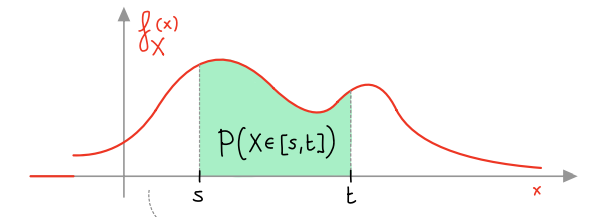
\includegraphics[scale=.7]{Foto/integrale.png} 
\end{figure}

\noindent \textbf{Osservazione}: Troviamo una analogia tra una variabile aleatoria discreta ed una assolutamente continua: $$ \text{V.A. discreta:} \sum_{x \in [s,t]} P_X(x_i) \qquad \text{V.A. assolutamente continua:} \int_s^t f_X(x) $$ 
 
\noindent Notiamo anche delle differenze importanti: se X è assolutamente continua $\forall x \in \mathbb{R}: P(X = x) = 0 $. In particolare, tranne per $f_X(x)=0$: $$f_X(x) \neq P(X = x)$$

\subsubsection{Densità}

La \textbf{densità} di una variabile aleatoria assolutamente continua X è una funzione $f_X: \mathbb{R} \xrightarrow{} \mathbb{R}$ integrabile tale che: $$ f_X(x) \geq 0 \quad \forall x \in \mathbb{R} \qquad \qquad \int_{-\infty}^{+\infty} f_X(x) dx = 1$$


\subsubsection{Valore medio e varianza di v.a. assolutamente continue}

Le definizioni di valore medio e varianza di v.a. assolutamente continue ricalcano quelle delle v.a. discrete:
\begin{itemize}
    \item $E[X] = \int_{-\infty}^{+\infty} x \cdot f(x) dx$
    \item $Var[X] = E[X^2] - E[X]^2$
    \item $Sd[X] = \sqrt{Var[X]}$
\end{itemize}
\noindent Anche le proprietà definite per le variabili discrete continuano a valere.

\subsection{Uniforme Continua}

Una variabile aleatoria X è \textbf{uniforme continua in [0,1]} e si indica con $X \sim U(0,1)$ se è definita da una funzione:
\begin{equation}
  f_X(x) =
    \begin{cases}
      c = 1& \text{se } x \in [0,1] \\
      0 & \text{se } x \not\in [0,1]\\
    \end{cases}       
\end{equation}

\noindent Una variabile aleatoria X è \textbf{uniforme continua in [a,b]} e si indica con $X \sim U(a,b)$ se è definita da una funzione:
\begin{equation}
  f_X(x) =
    \begin{cases}
      \dfrac{1}{b-a} = 1& \text{se } x \in [a,b] \\
      0 & \text{se } x \not\in [a,b]\\
    \end{cases}       
\end{equation}

\begin{figure}[h!]
    \centering
    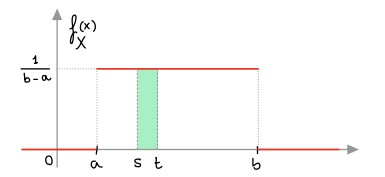
\includegraphics[scale=.8]{Foto/babu.jpg}
\end{figure}

\noindent Dato un intervallo $[s,t] \subseteq [a,b]$  avremo che $$P(X \in [s,t]) = \int_s^t f(x) dx + \dfrac{1}{b-a} = \int_s^t 1 \text{ } dx = \dfrac{t-s}{b-a}$$

\noindent \textbf{Osservazione}: Poiché la variabile aleatoria uniforme continua assume un'infinita quantità di valori in un intervallo continuo [0,3], la probabilità di ottenere un valore specifico x è zero. In altre parole, la probabilità di ottenere un risultato esatto in una variabile aleatoria continua è sempre zero. 

\subsection{Esponenziale}

Una variabile aleatoria \textbf{esponenziale} è spesso utilizzata per descrivere il tempo tra gli arrivi di eventi casuali indipendenti di un processo di Poisson. Misuriamo il tempo medio di evento come $\tau$, avremo che $\lambda = \dfrac{1}{\tau}$. La funzione che la descrive è

\begin{equation}
  f_X(x) =
    \begin{cases}
      \lambda \cdot e^{-\lambda \cdot x}& \text{se } x \geq 0\\
      0 & \text{se } x < 0\\
    \end{cases}       
\end{equation}

\begin{figure}[h!]
    \centering
    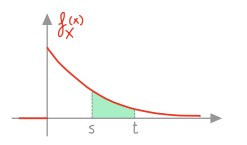
\includegraphics{Foto/bibi.jpg} 
\end{figure}

\noindent Una variabile aleatoria X con tale densità è detta esponenziale di parametro $\lambda \in (0, \infty) $ e si scrive X $\sim$ Exp($\lambda$). Avremo che:
\begin{itemize}
    \item $P(X \in [s,t]) = \int_s^t f_X(x)dx = e^{- \lambda \cdot s} - e^{- \lambda \cdot t}$
    \item $E[X] = \dfrac{1}{\lambda}$
    \item $Var[X] = \dfrac{1}{\lambda^2}$
\end{itemize}
\newpage
\subsection{Normale}

Abbiamo già visto due classi notevoli assolutamente continue: uniforme continua ed esponenziale. Consideriamo ora la più importante: \textbf{variabili aleatorie normali } (o gaussiane).

\noindent Una variabile aleatoria X si dice \textbf{normale standard} e si indica con \newline $Z \sim N(0,1)$ se è assolutamente continua e ha densità: $$f_Z(z) = \dfrac{1}{\sqrt{2 \cdot \pi}} \cdot e^{\left(-\dfrac{z^2}{2} \right)}$$

\begin{figure}[h!]
    \centering
    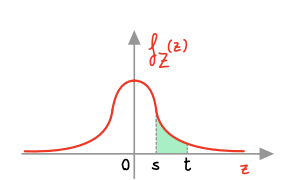
\includegraphics[scale=.8]{Foto/normale.png}
\end{figure}

\noindent Una variabile aleatoria normale standard avrà:
\begin{itemize}
    \item E[Z] = 0
    \item Var[Z] = 1 
    \item P(Z $\in [s,t]) = \displaystyle\int_s^t f_Z(z)dz$
\end{itemize}

\noindent Purtroppo l'integrabile non è calcolabile, allora si introduce la \textbf{funzione di ripartizione di Z} indicata con:  $$ \Phi(z) := F_Z(z) = P(Z \leq z) = \int_s^t f_Z(t)dt$$ Anche questa non è calcolabile esplicitamente ma i valori che può assumere sono riportati in una tabella. \newline

\begin{figure}[h!]
    \centering
    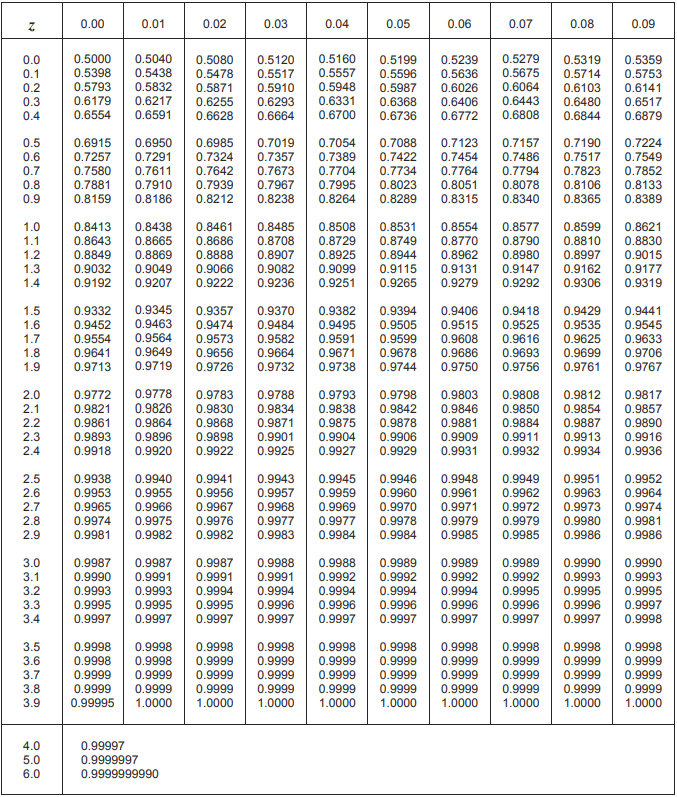
\includegraphics{Foto/tavolameglio.png}
\end{figure} 
\newpage
\noindent \textbf{Osservazione}: per valori negativi si applica la formula: $$\Phi(z) = 1 - \Phi(-z)$$

\newpage
\noindent Una variabile aleatoria X si dice \textbf{normale} con media $\mu$ e varianza $\sigma^2$ e si scrive con $X \sim N(\mu, \sigma^2)$ se X è assolutamente continua con: $$f_X(x) = \dfrac{1}{\sqrt{2 \cdot \pi \cdot \sigma^2}} \cdot e^{-\dfrac({z^2}{2})}$$

\begin{figure}[h!]
    \centering
    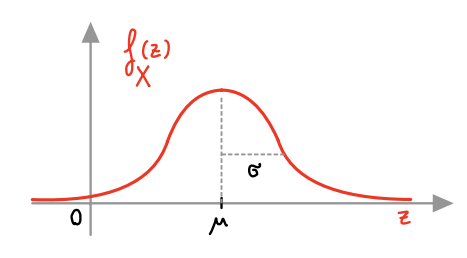
\includegraphics[scale=.7]{Foto/garfichino.png}
    \color{gray}
    \caption{grafico a campana centrato in $\mu$ di ampiezza $\sigma^2$}
\end{figure}

\noindent \textbf{Osservazione}: Ci si può sempre ricondurre da una variabile normale ad una normale standard e viceversa:
\begin{itemize}
    \item $X \sim N(\mu, \sigma^2) \rightarrow{} Z:= \dfrac{X - \mu}{\sigma} \sim N(0,1)$ 
    \item $Z \sim N(0,1) \xrightarrow{} X := \sigma \cdot Z + \mu \sim N(\mu, \sigma^2)$
\end{itemize}

\noindent \textbf{Osservazione}: Da questi trasformazioni, se abbiamo X v.a. normale standard, allora Z v.a. normale ha media $\mu$ e varianza $\sigma^2$: $$X \sim N(\mu, \sigma^2) \rightarrow{} E[Z] = \mu \quad Var[Z] = \sigma^2$$

\subsubsection{Teoremi}
Se X è normale, $Y = a \cdot X + b$ è normale. \newline Se X e Y sono normali indipendenti allora X + Y è normale

\begin{tcolorbox}
    \textbf{Esempio}: $X \sim N(0,1)$, $Y \sim N(0,1)$ allora $$X + Y \sim N(0,2) \qquad X - Y = X + (-1) \cdot (Y) \sim N(0,2)$$
\end{tcolorbox}

\subsubsection{Funzione di ripartizione}

Finora abbiamo studiato le v.a. discrete e assolutamente continue. Introduciamo un nuovo oggetto per v.a. generica: \textbf{funzione di ripartizione} $$F_X(x) := P(X \leq x)$$ 
\begin{itemize}
    \item $F_X$ è ben definita per ogni v.a.
    \item $F_X$ determina la distribuzione della v.a. X: $$P(X \in (s,t]) = F_X(t) - F_X(s)$$
    \item $F_X$ è legata alla densità discreta/densità di X: 
\begin{equation}
  F_X(x) =
    \begin{cases}
        \dsum_{x_i \in ( -\infty, x]} P_X(x_i) & \text{se x è discreta }\\
        \displaystyle\int_{-\infty}^x f_X(t)dt& \text{se x è assolutamente continua }\\
    \end{cases}       
\end{equation}
\end{itemize}

\begin{tcolorbox}
    \textbf{Esempio}: Funzione di ripartizione per variabile discreta: Bernoulli. \newline Sia $X \sim Be(p) \text{ con } p \in (0,1)$: $$X(\Omega) = \{0,1\} \qquad p_X(0) = 1 - p \qquad p_X(1) = p$$ Allora $F_X (x) = P(X \leq x)$ vale:
    \begin{equation}
        f_X(x) =
        \begin{cases}
            0 & \text{se } x < 0\\
            1 - p & \text{se } 0 \leq x < 1 \\
            1 & \text{se } x \geq 1
        \end{cases}       
    \end{equation}
    \end{tcolorbox}
    \begin{figure}[h!]
        \centering
        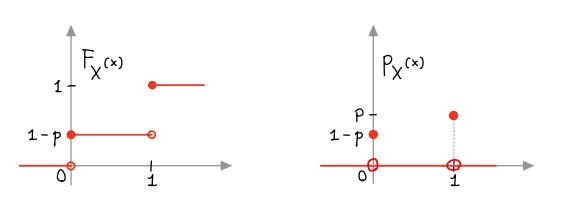
\includegraphics[scale=.6]{Foto/zaza.jpg} 
    \end{figure}


\begin{tcolorbox}
    \textbf{Esempio}: Funzione di ripartizione per variabile uniforme continua \newline Sia $X \sim U(a,b)$: $X(\Omega) = [a,b]$
    \begin{equation}
        f_X(x) = 
        \begin{cases}
            \dfrac{1}{b - a} & \text{ se } a \leq x \leq b \\
            0 & \text{ se } x < a \text{ o } x > b \\
        \end{cases}
    \end{equation}
    Allora $F_X(x) = P(X \leq x)$ vale:
    \begin{equation}
        F_X(x) =
        \begin{cases}
            0 & \text{ se } x < a \\
            \dfrac{x - a}{b - a} & \text{ se } a \leq x \leq b \\
            1  & \text{ se } x > b \\
        \end{cases}
    \end{equation}
\end{tcolorbox}
\begin{figure}[h!]
    \centering
    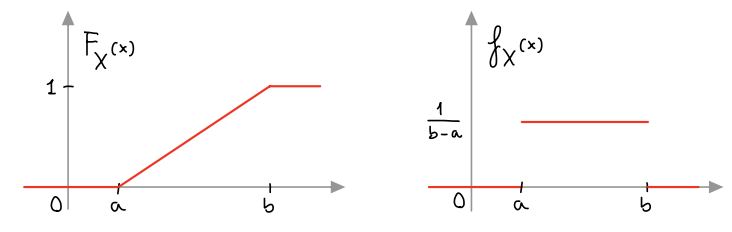
\includegraphics[scale=.7]{Foto/sium.png} 
\end{figure}

\noindent \textbf{Teorema di ripartizione di v.a. discrete} 
\begin{itemize}
    \item X è una variabile aleatoria discreta $\iff$ $F_X$ è costante a tratti 
    \item Valori assunti {$x_i$} $\iff$ punti di discontinuità di $F_X$ 
    \item Densità discreta $\iff$ ampiezze dei salti \item $P_X(x_i) = F_X(x_i) - F_X(x_{\Bar{i}}) $ dove $x_{\Bar{i}} = \lim_{t \xrightarrow{} x_{\Bar{i}}} F_X(t)$
\end{itemize} 

\noindent \textbf{Teorema di ripartizione di v.a. assolutamente continue}
\begin{itemize}
    \item X è una v.a. assolutamente continua (con densità continua a tratti) $\iff$ $F_X$ è una funzione continua ed è derivabile a tratti
    \item Densità $F_X (x) = (F_x)'(x)$
\end{itemize}

\section{Vettori Aleatori}

Abbiamo studiato le v.a. individualmente, ma spesso è interessante lo studio \textit{congiunto} di v.a. relative allo stesso esperimento aleatorio. 
\begin{equation}
  (\Omega, P) =
    \begin{cases}
      X: \Omega \xrightarrow{} \mathbb{R} & \text{variabile aleatoria}\\
      Y: \Omega \xrightarrow{} \mathbb{R} & \text{variabile aleatoria}\\
    \end{cases}       
\end{equation}
La coppia (X,Y) è detta \textbf{vettore aleatorio}: $$(X,Y) : \Omega \xrightarrow{} R^2$$

\subsection{Vettori Aleatori Discreti}

Un vettore $(X,Y)$ si dice \textbf{discreto} se i valori che può assumere sono contenuti in un insieme finito o numerabile $\{(x_i),(y_i)\}$ \newline

\noindent Si definisce \textbf{densità discreta congiunta} come: $$P_{(X,Y)}(x_i, Y_i) := P(X= x_i, Y=y_i) $$

\noindent La relazione tra densità discreta congiunta e la densità discreta delle singole variabili aleatorie è definita come \textbf{densità discreta marginale}: $$P_X(x_i) = \sum_{y_i} P_{(X,Y)}(x_i,y_i) \qquad P_Y(y_i) = \sum_{x_i} P_{(X,Y)}(x_i,y_i)$$

\noindent Il valore medio del prodotto tra due variabili aleatorie discrete X e Y è $$E[X,Y] = \sum_{x_i} \sum_{y_i} x_i \cdot y_i \cdot P_{X,Y}(x_i, y_i)$$

\begin{tcolorbox}
    \textbf{Esempio}: Lancio due monete dove X è prima moneta testa e Z numero totale di teste. \newline $X(\Omega) = {0,1}$ \newline $Y(\Omega) = {0,1,2} \newline p_{(X,Z)}(x,z) = P(X = x, Z = z)$ \newline
    
    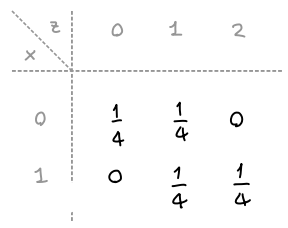
\includegraphics[scale=0.8]{Foto/vettore discreto.png}
\end{tcolorbox}

\subsection{Vettori Aleatori Assolutamente Continui}

Un vettore $(X,Y)$ si dice assolutamente continuo se esiste una funzione $f_{(X,Y)}(x,y) \geq 0$ detta \textbf{densità congiunta} di X e Y tale che $$P(X \in [s,t], Y \in [u,v]) = \int_s^t \left(\int_u^v f_{(X,Y)}(x,y) dy\right) dx$$

\noindent Si definiscono \textbf{densità marginali} come: $$f_X(x) = \int_{-\infty}^{+\infty} f_{(X,Y)}(x,y) dy \quad f_Y(y) = \int_{-\infty}^{+\infty} f_{(X,Y)}(x,y) dx$$

\noindent Il valore medio del prodotto tra due v.a. assolutamente continue X e Y è $$E[X \cdot Y] = \int_{-\infty}^{+\infty} \int_{-\infty}^{+\infty} x \cdot y \cdot f_{(X,Y)}(x,y) \text{ } dx  \text{ } dy$$

\subsection{Indipendenza}

Consideriamo due v.a. X e Y che insieme formano un vettore aleatorio (X,Y). Si dice che X e Y sono \textbf{indipendenti} se $$P(X \in [s,t], Y \in [u,v]) = P(X \in [s,t] \cdot Y \in [u,v])$$

\noindent  Da questa formula si può ricavare che X e Y sono indipendenti se conoscendo il valore che assume Y \textit{non cambia la distribuzione} di X: $$P(X \in [s,t] | Y \in [u,v] ) = P(X \in [s,t]$$

\noindent \textbf{Osservazione}: Per vettori discreti o assolutamente continui, l'indipendenza ha una riformulazione equivalente: $$(X,Y) \text{ discreto, X e Y sono indipendenti sse } p_{X,Y}(x_i,y_i) = p_X(x_i) \cdot p_Y(y_i)$$ $$(X,Y) \text{ assolut. continuo, X e Y sono indipendenti sse } f_{(X,Y)}(x,y) = f(x) \cdot f(y)$$

\noindent \textbf{Osservazione}: Quando le v.a. non sono indipendenti, le densità marginali forniscono meno informazioni della congiunta. Quando le v.a. sono dipendenti, le densità dei singoli fornisce la stessa quantità di informazioni della congiunta. \newline

\noindent Il valore medio del prodotto tra due variabili aleatorie indipendenti X e Y è $$E[X \cdot Y] = E[X] \cdot E[Y]$$

\subsection{Covarianza e Correlazione}

Consideriamo due v.a. X e Y che insieme formano un vettore aleatorio $(X,Y)$. Indichiamo i valori medi con $\mu_X = E[X]$ e $\mu_Y = E[Y]$. \newline Si definisce \textbf{covarianza} di X e Y: $$Cov[X,Y] := E[(X - \mu_X) \cdot (Y - \mu_Y)]$$

\noindent La covarianza misura il \textit{grado di associazione} tra X e Y: \newline $Cov[X,Y] > 0$: a valori grandi di X corrispondono valori grandi di Y \newline  $Cov[X,Y] < 0$: a valori grandi di X corrispondono valori piccoli di Y \newline

\noindent \textbf{Osservazione}: la covarianza si può riscrivere come $$Cov[X,Y] = E[X \cdot Y] - E[X] \cdot E[Y]$$

\subsubsection{Proprietà della covarianza}

\begin{itemize}
    \item Annullamento: $Var[X] = Cov[X, X]$
    \item Simmetria: $Cov[X,Y]= Cov[Y,X]$
    \item Costanti: $Cov[X, c] = 0$
    \item Bilinearità: $Cov[a \cdot X, Y] = a\cdot Cov[X, Y]$ 
    \item Bilinearità: $Cov[X + Z, Y] = Cov[X, Y] + Cov[Z, Y]$
    \item \textbf{Formula della somma}: $Var[X] + Var[Y] + 2 \cdot Cov[X,Y]$
\end{itemize}

\noindent Si definisce \textbf{coefficiente di correlazione lineare}: $$\rho[X,Y] := \dfrac{Cov[X,Y]}{Sd[X] \cdot Sd[Y]}$$ Si tratta di una versione normalizzata della covarianza: 
\begin{itemize}
    \item $-1 \leq \rho[X,Y] \leq 1$
    \item $\rho = \pm 1 \longleftrightarrow Y = a \cdot X + b$
\end{itemize}

\noindent Se Cov[X,Y] = 0, X e Y si dicono \textbf{scorrelate}. \newline

\noindent \textbf{Osservazione}:  Se abbiamo due variabili aleatorie indipendenti, allora sicuramente sono scorrelate, ma \textit{non vale viceversa}

\begin{tcolorbox}
    \textbf{Esempio}: Lancio due dadi regolari a 6 facce. Siano X la somma dei risultati e Y la differenza. Allora X e Y sono scorrelate:
    \begin{equation}
      \begin{aligned}
        Cov[X, Y] & = Cov[A+B, A-B]\\
          & = Cov[A,A] - Cov[A,B] - Cov[B,A] - Cov[B,B]\\
          & = Cov[A,A] - Cov[B,B] \\
          & = Var[A] - Var[B] = 0 
      \end{aligned}
    \end{equation}
    Tuttavia X e Y non sono indipendenti. Per esempio: $$P(X = 12) = \dfrac{1}{6} \quad P(Y = 5) = \dfrac{1}{6}$$ $$P(X = 12, Y = 5) = 0$$ $$ 0 \not= \dfrac{1}{6} \cdot \dfrac{1}{6}$$
\end{tcolorbox}

%-------------Introduzione alla Statistica -----------------------%
\begin{comment}
\section{Verso la Statistica}

Il modello fondamentale per la statistica è una \textbf{sucessione di variabili aleatorie indipendenti e identicamente distribuite (I.I.D.)} \newline

\noindent In un esperimento concreto si osserva una successione di dati numerici $x_1 \cdots x_N$ che interpretiamo come realizzazioni di variabile aleatorie $X_1 \cdots X_N$. \newline 

\noindent Ci poniamo il problema: a partire dai dati $x_1 \cdots x_N$ cosa possiamo dedurre sulla \textit{distribuzione comune} delle v.a. $X_i$?
\end{comment}
%----------------------------------------------------------------%








\chapter{Teoremi di Convergenza}

\section{Teoria}

\subsection{Campione Aleatorio Casuale}

Il modello probabilistico fondamentale per la statistica è la successione $\suc$ di variabili aleatorie \textbf{indipendenti ed identicamente distribuite} (v.a i.i.d.) \n

\ind \textbf{Definizione}: Chiameremo \textbf{campione aleatorio casuale} di ampiezza n le $\suc$ osservabili. \n 

\ind \textbf{Osservazione}: Uno dei pochi casi in cui è facile conoscere la distribuzione del campione aleatorio è il caso del \textbf{campione gaussiano} $\suc \sim N(\mu, \sigma^2)$ in quanto possiamo calcolare la media campionaria $\mc $ con la tavola della distribuzione. \n

\ind \textbf{Obiettivo}: Per ottenere il nostro obiettivo, ovvero quello di conoscere la distribuzione di un campione aleatorio $\suc$, dovremo ricondurre il campione aleatorio ad una gaussiano $N(0,1)$ \n

\ind \textbf{Definizione}: Per standardizzare un campione aleatorio $\suc$ dovremo prendere la somma di tale campione, sottrarre la sua media e dividere per la radice della varianza: $$\std$$

\newpage
\ind \textbf{Osservazioni}: Guardiamo ora le distribuzioni di $\suc $ per campioni non normali. Avremo che le densità si riconducono a quella di una normale \textit{all'aumentare di n}.\n
\begin{figure}[h!]
    \centering
    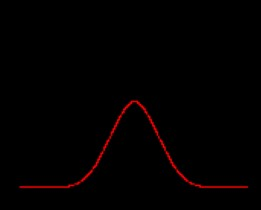
\includegraphics[scale=0.7]{Foto/uc.jpg}
    \color{gray}
    \caption{Uniforme Continua di parametro $U(0,1)$ con n=16}
    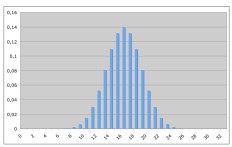
\includegraphics[scale=.9]{Foto/be.jpg}
    \color{gray}
    \caption{Bernoulli di parametro $Be(\sfrac{1}{2})$ con n=32}
    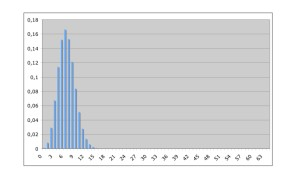
\includegraphics[scale=.8]{Foto/be110.jpg}
    \color{gray}
    \caption{Bernoulli di parametro $Be(\sfrac{1}{10})$ con n=64}
\end{figure}

\newpage
\subsection{Teorema del Limite Centrale}

\ind \textbf{Definizione}: Il \textbf{Teorema del Limite Centrale} (TLC) afferma che la somma o la media di un grande numero di v.a. i.i.d e è approssimativamente normale per n grande ($n \geq 30$). Siano $E[X_i]=\mu$ e $Var[X_i]=\sigma^2$ allora $$ \text{Media: } \pP \left( \dfrac{\mc - \mu}{ \dfrac{\sigma}{\sqrt{n}}} \leq x \right) \sim P(Z \leq x)$$ $$ \text{Somma: } \pP \left( \dfrac{\somsuc - \mu}{ \sigma} \leq x \right) \sim P(Z \leq x)$$

\subsection{Correzioni di Continuità}

\ind \textbf{Definizione}: La correzione di continuità si applica quando si standardizza una distribuzione discreta ad una normale. Afferma che bisogna ampliare di $\sfrac{1}{2}$ gli estremi dell'intervallo per ottenere un valore ben approssimato \n

\ind \textbf{Definizione}: La correzione di continuità di una \textbf{binomiale} afferma che dato se $np \geq 5$ e $n(1 - p) \geq 5$ allora la sua correzione è $$X \sim Bin (np, np(1 - p))$$ 

\ind \textbf{Definizione}: Se non ci troviamo nel caso di prima, quindi $np \leq 5$ e $n(1 - p) \leq 5$ allora approssimiamo con la correzione di continuità di una \textbf{Poisson}: $$X \sim Pois(n(1 - p))$$

%%%%%%%%%%%%%%%%%%%%%%%%%%%%%%%%%%%%%%%%%%%%%%%%%%%%%%%%%%%%%%%%%%%%%%%%%%%%%%%%%%%%%%%%%%%%%%%%%%%%%%%%%%%%%%%%%%%%%%%%%%%%%%%

\newpage
\section{Pratica}

\ind \textbf{Standardizzazione}: $\std$ \n

\ind \textbf{TLC}: $$ \text{Media: } \pP \left( \dfrac{\mc - \mu}{ \dfrac{\sigma}{\sqrt{n}}} \leq x \right) \sim P(Z \leq x)$$ $$ \text{Somma: } \pP \left( \dfrac{\somsuc - \mu}{ \sigma} \leq x \right) \sim P(Z \leq x)$$

\ind \textbf{CC}: Riduzione di $\sfrac{1}{2}$ del dominio per approssimare V.A. discrete \n

\ind \textbf{CC Binomiale}: se $np \geq 5$ e $n(1 - p) \geq 5$ allora: $X \sim Bin (np, np(1 - p))$ \n

\ind \textbf{CC Poisson}: se $np \leq 5$ e $n(1 - p) \leq 5$ allora: $X \sim Pois(n(1 - p))$

\subsection{Esercizi} 

\subsubsection{Esercizio 1: TLC con assolutamente continua}

\textbf{Traccia}: Una lampada ha un tempo di vita che segue una legge esponenziale di media 10 giorni. Non appena la lampada smette di funzionare, viene sostituita con una nuova. 
\begin{enumerate}
    \item [a. ] Qual è la probabilità che 40 lampade siano sufficienti per un anno?
    \item [b. ] Qual è il numero minimo n di lampade comprare affinché la probabilità dell'evento "n lampade siano sufficienti per un anno" sia almeno 0.95?
\end{enumerate} 

\ind \textbf{Soluzione a}: 
\begin{enumerate}
    \item Ricavo dalla traccia che ho 40 lampade con legge esponenziale di media 10 giorni. Ricavo dalla tabella che se $E[X]=\sfrac{1}{\lambda}=10$, allora $\lambda=\sfrac{1}{10}$ Riscrivo come $X_1, ..., X_{40}$ v.a. i.i.d. $\sim exp(\sfrac{1}{10})$
    \item La richiesta è $\pP (X_1 + ... + X_{40} > 365)$. Dato che $n=40$ è abbastanza grande, possiamo stimare questa probabilità con il TLC.
    \item Dobbiamo standardizzare la somma delle nostre v.a. Per farlo abbiamo bisogno di conoscere valore medio $E[X] = \sfrac{1}{\lambda}$ e varianza $Var[X] = \sfrac{1}{\lambda^2}$: 
        \begin{itemize}
            \item Per la linearità della media, $E[X+Y] = E[X] + E[Y]$: $$E[X_1 + ... + X_{40}] = E[X_1] + ... + E[X_{40}] = 10 + ... + 10 = 400$$
            \item Per l'indipendenza delle v.a., $Cov[X+Y]=0$ quindi $Var[X+Y]= Var[X] + Var[Y]$: $$Var[X_1 + ... + X_{40}] = Var[X_1] + ... + Var[X_{40}] = 100 + ... + 100 = 4000$$
        \end{itemize}
    \item Standardizziamo con la formula: $\std$: $$\pP (X_1 + ... + X_{40} > 365) = \pP \left( \dfrac{X_1 + ... + X_{40} - 400}{\sqrt{4000}} > \dfrac{365 - 400}{\sqrt{4000}} \right) $$
        \begin{itemize}
            \item Semplifichiamo e cambiamo $>$ in $\leq$: $$= 1 - \pP \left( \dfrac{X_1 + ... + X_{40} - 400}{\sqrt{4000}} \leq \dfrac{-35}{20\sqrt{10}} \right)$$
            \item Essendo $\sim N(0,1)$ usando il TLC avremo: $$\simeq 1 - \pP \left(Z \leq  \dfrac{-35}{20\sqrt{10}} \right) = 1 -\Phi \left( \dfrac{-35}{20\sqrt{10}} \right)$$  
            \item Essendo l'argomento negativo diventa: $$1 - 1 - \Phi \left( \dfrac{35}{20\sqrt{10}} \right) = \Phi(0.55) = 0.7088$$
        \end{itemize}
    \item La probabilità che 40 lampade siano sufficienti per un anno è 71\%
\end{enumerate}

\ind \textbf{Soluzione b}:
\begin{enumerate}
    \item Abbiamo $X_1 + ... + X_n \sim exp(\sfrac{1}{10})$. L'incognita ora è n. Cerchiamo il minimo n  tc $ \pP(X_1 + ... X_N > 365) \geq 0.95)$
    \item Sicuramente n deve essere $>$ 40 in quanto al punto a. dava probabilità 0.71 e a noi serve 0.95. Essendo n grande, il TLC è applicabile con buona approssimazione.
    \item Dobbiamo standardizzare la somma delle nostre v.a. Calcoliamo valore medio e varianza:
        \begin{itemize}
            \item $E[X_1 + ... + X_n] = E[X_1] + ... + E[X_n] = 10n$
            \item $Var[X_1 + ... + X_n] = Var[X_1] + ... + Var[X_n] = 100n$
        \end{itemize}
    \item Standardizzo: $$ \pP(X_1 + ... + X_n > 365) = 1 - \pP \left( \dfrac{X_1 + ... + X_{n} - 10n}{\sqrt{100n}} \leq \dfrac{365 - 10n}{\sqrt{10\sqrt{n}}} \right)$$
    \item Avrò numeratore negativo perché $n>40$ quindi per TLC: $$\Phi\left(\frac{10n - 365}{10 \sqrt{n}}\right)$$
    \item Calcoliamo il minimo n tc. $$\Phi \left(\frac{10n - 365}{10 \sqrt{n}}\right) \geq 0.95$$
    \item Calcolo con la fdr lo $z^*$ tc $\Phi(z^*) = 0.95$ e trovo $\Phi(1.645)$: $$\Phi\left( \frac{10n - 365}{10 \sqrt{n}}\right) \geq \Phi(1.645) =  \frac{10n - 365}{10 \sqrt{n}} \geq 1.645= \qquad (\sqrt{n} = x)$$  $$= 10x^2 - 16.45x - 365 \geq 0 \xrightarrow{} x=6.92= n \sim 47.89$$ 
    \item Il minimo numero di lampadine da compare è 48
\end{enumerate}

\subsubsection{Esercizio 2: TLC con discreta + CC }

\textbf{Traccia}: Qual è la probabilità di ottenere almeno 29 teste in 50 lanci di una moneta equilibrata? \n

\ind \textbf{Soluzione}: 
\begin{enumerate}
    \item Definiamo $X_1, ..., X_{50} $ v.a. i.i.d $\sim Be(\sfrac{1}{2})$
    \item Cerco il numero di teste nei 50 lanci: $\pP(X_1 + ... + X_{50} \geq 29) $, ovvero $Bin(50, \frac{1}{2})$ con numero di successi $k=29$
    \item Devo usare la CC di una binomiale, dunque devo rispettare due condizioni:
        \begin{enumerate}
            \item $np \geq 5$: $np=50 \cdot \sfrac{1}{2}= 25 \geq 5$
            \item $n(1-p) \geq 5$: $n(1-p)=50\cdot \sfrac{1}{2}=25 \geq 5$
        \end{enumerate}
    \item Essendo entrambe le condizioni confermate, posso approssimare con una binomiale della forma: $$X \sim Bin(np, np(1-p)) = Bin(25, \sfrac{25}{2})$$
    \item Approssimo con la CC ed ottengo: $$\pP(X_1 + ... + X_{50} \geq 28.5) = \pP \left( \dfrac{X_1 + ... + X_{50} - 25}{\sqrt{\dfrac{25}{2}}} \right)$$
    \item Applico il TLC: $$\pP(X_1 + ... + X_{50} \geq 28.5) \sim 1 - \pP \left(Z \leq \frac{7}{\sqrt{50}} \right) = 1 - \Phi(0.99) = 0.1611$$
    \item La probabilità di ottenere almeno 29 teste in 50 lanci è del 16\%
\end{enumerate}




\chapter{Statistica Inferenziale}

\section{Teoria}

\subsection{Introduzione}

\textbf{Definizione}: La \textit{statistica inferenziale} consente di dedurre particolari caratteristiche di una popolazione limitandosi ad analizzare un numero finito e preferibilmente piccolo di suoi individui. \n

\ind \textbf{Definizione}: Quando le caratteristiche che si vogliono individuare sono esprimibili numericamente allora esse sono dette \textit{parametri}. \n

\ind \textbf{Definizione}: Per \textit{stima di parametri} si intende quindi il problema della deduzione di parametri di una popolazione facendo ricorso all’analisi di un suo
sottoinsieme finito opportunamente scelto, detto \textit{campione}. \n

\ind \textbf{Osservazione}: Diverse tecniche possono essere utilizzate per effettuare delle stime di parametri. Noi ci limiteremo a considerare quelle classiche basate sulla conoscenza delle \textit{distribuzioni campionarie}. \n

\ind \textbf{Definizione}: Diverse ragioni possono portare a voler determinare le caratteristiche di una popolazione facendo ricorso esclusivamente ad un numero limitato di suoi individui: tempo, costo, disponibilità ecc. In questi casi occorre allora effettuare un \textit{campionamento}, ovvero una scelta degli individui che verranno analizzati per effettuare le inferenze sull’intera popolazione. \n

\ind \textbf{Osservazione}: Tutte le tecniche che verranno presentate in questo capitolo sono valide solo nel caso in cui il campione sia stato scelto secondo una procedura detta \textit{campionamento casuale}. \n

\ind \textbf{Definizione}: Denotiamo con X il \textit{carattere} della popolazione su cui siamo interessati a fare dell’inferenza. Penseremo ad X come ad una \textit{variabile aleatoria} la cui \textit{distribuzione sconosciuta} corrisponde a quella che si otterrebbe facendo ricorso alle tecniche della statistica descrittiva sull'intera popolazione, e pensare invece ai valori assunti dai singoli individui come a delle \textit{realizzazioni} di X. In forma matematica:
\begin{itemize}
    \item Campione casuale di numerosità n $(X_1, X_2, ..., X_n)$ : è una n-pla di v.a indipendenti aventi ognuna la stessa distribuzione del carattere X della popolazione. 
    \item I valori $(x_1, x_2, ..., x_n) $ assunti dalla n-pla sono una realizzazione di $(X_1, X_2, ..., X_n)$.
\end{itemize}

\subsection{Stime Puntuali}

\textbf{Definizione}: Possiamo pensare al carattere della popolazione su cui vogliamo fare delle inferenze come ad una variabile aleatoria X, avente una \textit{funzione di ripartizione F sconosciuta}, ma corrispondente alla distribuzione di frequenza cumulata di tale carattere, che si potrebbe ottenere se fosse possibile analizzare per intero la popolazione. \n

\ind \textbf{Definizione}: Una \textit{stima} è una realizzazione di una statistica campionaria. \n

\ind \textbf{Osservazione}: Per le prossime definizioni denoteremo con $\mu$ il valore atteso e con $\sigma^2$ la varianza della popolazione X con distribuzione F incognita. \n

\ind \textbf{Definizione}: Uno stimatore si dice \textit{non distorto} se il loro valore atteso è uguale al valore medio che vogliamo stimare: $$E[T]_{\Theta} = E[g(\suc)]_{\Theta} = \Theta$$ Questa proprietà non è stabile a trasformazioni non lineari. Uno stimatore non distorto si dice \textit{consistente} quando ha varianza che tende a 0 con N grande. \n

\ind \textbf{Definizione}: Considerato un campione $(X_1, X_2, ..., X_n)$ estratto da una popolazione X, con distribuzione F, media $\mu$ e varianza $\sigma^2$ incognite. Definiamo \textit{media campionaria} la variabile: $$\mc : \frac{X_1 + X_2 + ... + X_n}{n}$$ Questo stimatore è non distorto in quanto $E[\mc]=\mu$. \n

\ind \textbf{Definizione}: Considerato un campione $(X_1, X_2, ..., X_n)$ estratto da una popolazione X, con distribuzione F, media $\mu$ e varianza $\sigma^2$ incognite. Definiamo \textit{varianza campionaria} la variabile: $$\sn = \dfrac{1}{n} \sum_{i=1}^n(X_i - \mc) $$ Questo stimatore è non distorto in quanto $E[\sn]=\sigma^2$. \n

\ind \textbf{Definizione}: Considerato un campione $(X_1, X_2, ..., X_n)$ estratto da una popolazione X, con distribuzione F, media $\mu=E[X_i]$ nota e varianza $\sigma^2$ incognita. Definiamo \textit{varianza campionaria} la variabile: $$\sn = \dfrac{1}{n} \sum_{i=1}^n(X_i - \mu) $$ Questo stimatore è non distorto in quanto $E[\overline{\sn}]=\sigma^2$. \n

\subsection{Distribuzione delle Statistiche Campionarie}

\ind \textbf{Definizione}: Prendiamo una v.a. i.i.d $Z \sim N(\mu, \sigma^2)$ e $\alpha \in (0,1)$. Si definisce $z_{\alpha} $ quel valore tale che $$\pP(Z > z_{\alpha}) =\alpha$$ 

\ind \textbf{Osservazione}: Vale anche $z_{\alpha} = - z_{1 - \alpha}$ \n

\ind \textbf{Definizione}: Siano $Z_1, ..., Z_n \sim N(0,1)$. Allora introduciamo  Y come una distribuzione \textit{chi quadrato con n gradi di libertà} tale che  $$Y=\sum_{i=1}^n Z_i^2 \sim \chiqm$$

\ind \textbf{Definizione}: Per $\alpha$ si pone $x^2_{n, \alpha}$ quel valore tale che: $$\pP (Y > x^2_{n, \alpha}) = \alpha$$

\ind \textbf{Osservazioni}:
\begin{itemize}
    \item si ha $E[Y]=n, Var[Y]= 2n$ 
    \item per n = 2 è la legge di $exp(\sfrac{1}{2})$
    \item per n grande vale l'approssimazione della legge con una $N(n, 2n)$
\end{itemize}

\ind \textbf{Definizione}: Sia $\mc$ un campione casuale estratto da una popolazione $N(\mu, \sigma^2)$:
\begin{enumerate}
    \item $\dsum_{i=1}^n \left( \dfrac{x_i - \mu}{\sigma} \right)^2 \sim \chiqm$
    \item $\dsum_{i=1}^n \left( \dfrac{x_i - \mc}{\sigma} \right)^2 \sim \chiqmn$
    \item se $\sn = \dfrac{1}{n-1} \dsum_{i=1}^n \left( \dfrac{X_i - \mc}{\sigma} \right) ^2$ allora $(n -1) \dfrac{\sn}{\sigma^2} \sim \chiqmn$
\end{enumerate}

\ind \textbf{Osservazione}: Osservando i punti 1) e 2), posiamo notare che ogni volta che stimiamo un parametro con chi quadrato, perdiamo un grado di libertà \n

\ind \textbf{Definizione}: Siano $Z \sim N (0, 1), Y \sim \chiqm$ indipendenti, definiamo T come una distribuzione \textit{ t di Student con n gradi di libertà} come: $$T= \dfrac{Z}{\sqrt{\sfrac{ Y}{n}}} \qquad T \sim t(n)$$

\ind \textbf{Definizione}: Per $\alpha$ si pone $t_{n, \alpha}$ quel valore tale che: $$\pP (T > t_{n, \alpha}) = \alpha$$

\ind \textbf{Osservazione}: T è simmetrica rispetto a 0. Quindi $t_{\alpha, n} = t_{1 - \alpha, n}$

\subsection{Stima per Intervalli}

Abbiamo visto come trovare un valore approssimato di un parametro incognito della popolazione per mezzo di una stima puntuale. Tali stime però non forniscono informazioni sul grado di approssimazione delle stesse. Per questo motivo alle stime puntuali vengono preferite quando possibile determinarle le \textit{stime per intervalli} che sono stime espresse sotto forma di \textit{intervalli fiduciari} all’interno dei quali con buona probabilità si trova il valore vero del parametro da stimare. \n

\ind \textbf{Definizione}: Definiamo $\alpha \in [0,1]$ come \textit{livello di confidenza} della stima ed il corrispondente intervallo è detto \textit{intervallo di confidenza}. Spesso $\alpha$ assume come valori 0.1, 0.05 e 0.01 . \n


\ind \textbf{Definizione}: La \textit{stima intervallare della media} di un campione estratto da una popolazione normale con \textit{media incognita e varianza nota pari a $\sigma^2$} ha come intervallo di confidenza: $$IC =  \left( \overline{x_n} - z_{\sfrac{\alpha}{2}} \dfrac{\sigma}{\sqrt{n}}, \overline{x_n} + z_{\sfrac{\alpha}{2}} \dfrac{\sigma}{\sqrt{n}} \right) $$

\ind \textbf{Osservazione}: L'ampiezza dell'intervallo è due volte l'errore, ovvero lo scarto dal valore centrato. Nell'esempio di stima della media con media incognita e varianza nota, l'ampiezza è: $$2 z_{\sfrac{\alpha}{2}} \cdot \frac{\sigma}{\sqrt{n}}$$


\ind \textbf{Osservazione}: La bontà della stima dipende dal livello di confidenza: maggiore è, più affidabile è la stima; ma all'aumentar di quest'ultimo, aumenta l'ampiezza dell'intervallo e quindi meno precisa sarà la stima. \n

\ind \textbf{Definizione}: La \textit{stima intervallare della media} di un campione estratto da una popolazione normale con \textit{media e varianza incognita} utilizza la t di Student con n-1 gradi di libertà. Ha come intervallo di confidenza: $$IC =  \left( \overline{x_n} - t_{n-1,\frac{\alpha}{2}} \dfrac{s_n}{\sqrt{n}}, \overline{x_n} + t_{n-1,\frac{\alpha}{2}} \dfrac{s_n}{\sqrt{n}}\right) $$

\ind \textbf{Definizione}: La stima proporzione-frequenza di una popolazione \textit{Bernoulliana} con media e varianza incognite, valida se $n\overline{x_n} > 5$ e $n(1 - \overline{x_n}) >5$ ha come intervallo di confidenza: $$IC = \left(\overline{x_n} - z_{\sfrac{\alpha}{2}} \sqrt{\dfrac{\overline{x_n}(1 -\overline{x_n})}{n}}, \overline{x_n} + z_{\sfrac{\alpha}{2}} \sqrt{\dfrac{\overline{x_n}(1 -\overline{x_n})}{n}} \right) \qquad \overline{x_n}(1 -\overline{x_n}) \leq \dfrac{1}{4}$$

\ind \textbf{Definizione}: Stima intervallare della \textit{varianza} su un campione estratto da una popolazione normale con media e varianza incognite è: $$IC =  \left( \dfrac{(n-1) s_n^2}{ \chi_{n-1, \sfrac{\alpha}{2}}}, \dfrac{(n-1) s_n^2}{ \chi_{n-1, \sfrac{ 1 - \alpha}{2}}} \right)$$

\ind \textbf{Definizione}: Stima intervallare della \textit{varianza} su un campione estratto da una popolazione normale con media nota e varianza incognita utilizza una $\chi$ con n-1 gradi di libertà ed è: $$IC = \left( \dfrac{n \overline{s_n^2}}{ \chi_{n, \sfrac{\alpha}{2}}}, \dfrac{n \overline{s_n^2}}{ \chi_{n, \sfrac{ 1 - \alpha}{2}}} \right)$$
\pagebreak 

\section{Pratica}

\subsection{Esercizi}

\subsubsection{Esercizio 1: Intervalli di Confidenza, Stime Media}

\textbf{Traccia}: La concentrazione di PCB nel latte materno ha approssimativamente una distribuzione Normale con media $\mu$ e varianza $\sigma^2$ entrambe incognite. Si misura un campione di 20 individui, ottenendo $\overline{x_n}=5.8$ e $s_n=5.085$
\begin{enumerate}
    \item IC per $\mu$ a livello 95\%
    \item IC per $\mu$ a livello 99\%
    %\item Come cambia il punto 1. se abbiamo varianza nota pari a 25?
\end{enumerate}

\ind \textbf{Soluzione punto 1}: 
\begin{enumerate}
    \item \textit{Trovo la formula da usare}: sono nel caso di media e varianza incognite e voglio trovare l'intervallo di $\mu$, controllo nel formulario delle stime per intervalli e trovo: $$ IC = \left( \mc - t_{n-1,\frac{\alpha}{2}} \dfrac{s_n}{\sqrt{n}}, \mc + t_{n-1,\frac{\alpha}{2}} \dfrac{s_n}{\sqrt{n}}\right) $$
    \item \textit{Calcolo $\alpha$}: Abbiamo $100(1 - \alpha)\% = 95\%$. Trovo $\alpha=0.05$
    \item \textit{Riscrivo i miei dati}: Ho $n=20$, $\overline{x_n}=5.8$, $s_n=5.085$, $\alpha=0.05$. Riguardando la formula mi manca conoscere $\frac{\alpha}{2}=0.025$
    \item \textit{Uso la tavola di t di Student}: Incrocio $n-1=19$ e $\frac{\alpha}{2}=0.025$ e trovo 2.093
    \item \textit{Riscrivo la formula}: $$IC = \left( 5.8 - 2.093 \frac{5.085}{\sqrt{20}}, 5.8 + 2.093 \frac{5.085}{\sqrt{20}} \right) \simeq (3.12 , 8.18)$$
    \item \textit{Conclusione}: L'intervallo di confidenza per $\mu$ a livello 95\% è $(3.12 , 8.18)$ 
\end{enumerate}

\ind \textbf{Soluzione punto 2}: 
\begin{enumerate}
    \item \textit{Trovo la formula da usare}: Sono nello stesso caso di prima in quanto cambia solo il livello di confidenza $$ IC = \left( \mc - t_{n-1,\frac{\alpha}{2}} \dfrac{s_n}{\sqrt{n}}, \mc + t_{n-1,\frac{\alpha}{2}} \dfrac{s_n}{\sqrt{n}}\right) $$
    \item \textit{Calcolo $\alpha$}: A differenza del precedente punto, adesso ho un livello di 99\% quindi $100(1 - \alpha)\% = 99\%$. Trovo $\alpha=0.01$
    \item \textit{Riscrivo i miei dati}: Ho $n=20$, $\overline{x_n}=5.8$, $s_n=5.085$, $\alpha=0.01$. Riguardando la formula mi manca conoscere $\frac{\alpha}{2}=0.005$
    \item \textit{Uso la tavola di t di Student}: Incrocio $n-1=19$ e $\frac{\alpha}{2}=0.005$ e trovo 2.861
    \item \textit{Riscrivo la formula}: $$IC = \left( 5.8 - 2.861 \frac{5.085}{\sqrt{20}}, 5.8 + 2.861 \frac{5.085}{\sqrt{20}} \right) \simeq (2.55 , 9.05)$$
    \item \textit{Conclusione}: L'intervallo di confidenza per $\mu$ a livello 95\% è $(2.55 , 9.05)$
\end{enumerate}

%\ind \textbf{Soluzione punto 3}:
%\begin{enumerate}
 %   \item \textit{Trovo la formula da usare}: Adesso siamo nel caso in cui media è incognita ma la varianza è nota ed è pari a 25. La formula da usare sarà: $$ IC = \left( \overline{x_n} - z_{\sfrac{\alpha}{2}} \dfrac{\sigma}{\sqrt{n}}, \overline{x_n} + z_{\sfrac{\alpha}{2}} \dfrac{\sigma}{\sqrt{n}} \right) $$
 %   \item \textit{Uso la tavola della Normale}: Trovo con la tavola della Normale che $z_{\sfrac{\alpha}{2}}=z_{0.025}$ e quindi devo trovare $\pP(Z \leq z_{0.025})= 1 - 0.025 = 0.975$ Trovo quindi $z_{0.025}=1.96$
  %% \item \textit{Conclusione}: Con varianza nota pari a 25, l'intervallo è aumentato.
%\end{enumerate}

\subsubsection{Esercizio 2: Intervalli di Confidenza, Stime Proporzioni}

\textbf{Traccia}: Voglio stimare la proporzione di donne tra gli insegnanti della scuola secondaria. Su un campione di 1000 insegnanti ci sono 518 donne.
\begin{enumerate}
    \item Stima puntuale della popolazione tramite uno stimatore non distorto
    \item IC al 95\% della proporzione
    \item IC al 99\% la cui ampiezza non sia maggiore di 0.03. Quanto dovrebbe essere numeroso il campione?
\end{enumerate}

\ind \textbf{Soluzione Punto 1}: Siamo nel caso campione numero estratto da una popolazione Bernoulliana Be(p) con p incognito e quindi media e varianza incognite. Uno stimatore non distorto di una Be(p) è la media p. Dunque la stima puntuale richiesta è $ \overline{x_n} = \sfrac{518}{1000}= 0.518$ \n 

\ind \textbf{Soluzione Punto 2}:
\begin{enumerate}
    \item \textit{Trovo la formula da usare}: Dal formulario, $$IC = \left(\overline{x_n} - z_{\sfrac{\alpha}{2}} \sqrt{\dfrac{\overline{x_n}(1 -\overline{x_n})}{n}}, \overline{x_n} + z_{\sfrac{\alpha}{2}} \sqrt{\dfrac{\overline{x_n}(1 -\overline{x_n})}{n}} \right)$$
    \item \textit{Trovo $\alpha$}: $z_{\sfrac{\alpha}{2}} $ è il $100(1 - \sfrac{\alpha}{2})$esimo percentile quindi $\alpha=0.05$ e $\sfrac{\alpha}{2}=0.025$
    \item \textit{Tavola Gaussiana}: A differenza della t Student, non troviamo la coda, ma la fdr. Quindi dobbiamo trovare $P( Z \leq z_{0.025}) = 1 - 0.025 = 0.975$ e quindi trovo che $z_{0.025}=1.96$
    \item \textit{Riscrivo la formula}: $$IC= \left( 0.518 - 1.96 \sqrt{\dfrac{0.518(1-0.518)}{1000}}, 0.518 + 1.96 \sqrt{\dfrac{0.518(1-0.518)}{1000}} \right)$$  $$\simeq (0.487, 0.549)$$
    \item \textit{Conclusione}: L'intervallo di confidenza per la proporzione a livello 95\% è $(0.487, 0.549)$
\end{enumerate}

\ind \textbf{Soluzione Punto 3}:
\begin{enumerate}
    \item \textit{Formula Ampiezza}: L'ampiezza di un IC per definizione è 2 volte lo scarto:  $$2 z_{\sfrac{\alpha}{2}} \sqrt{\dfrac{\overline{x_n}(1 -\overline{x_n})}{n}}$$ 
    \item \textit{Ricavare i dati}: Non conosciamo $\overline{x_n}(1 -\overline{x_n})$, ma è sicuramente $\leq \sfrac{1}{4}$ (vedi da formulario). La formula diventa $$2 z_{\sfrac{\alpha}{2}} \sqrt{\dfrac{\sfrac{1}{4}}{n}} = z_{\sfrac{\alpha}{2}} \frac{1}{\sqrt{n}} $$
    \item \textit{Tavola Gaussiana}: Dato $\sfrac{\alpha}{2}=0.005$ devo trovare nella tavola $0.995$ e lo incastro tra i valori $(2.57, 2.58)$ quindi $z_{0.005}=2.575$
    \item \textit{Riscrivo la formula}: $$ 2.575 \frac{1}{\sqrt{n}} \leq 0.03 \xrightarrow{} \sqrt{n} \geq \dfrac{2.575}{0.03} \xrightarrow{} n \geq 7373.08$$
    \item \textit{Conclusione}: Per avere IC al 99\% con ampiezza non maggiore di 0.03 ho bisogno di 7374 professori
\end{enumerate}

\subsubsection{Esercizio 3: Intervalli di Confidenza, Stime Varianza}

\textbf{Traccia}: Si considera il campione  
\begin{center}
    1.75 2.25 1.9 2.3 2.1 1.7
\end{center}
proveniente da una legge normale con media e varianza incognite.
\begin{enumerate}
    \item Stima puntuale della varianza usando stimatore non distorto
    \item IC al 99\% per $\sigma^2$
    \item Come cambiano le risposte se $\mu$ è nota pari a 2
\end{enumerate}

\ind \textbf{Soluzione Punto 1}: Stimatore non distorto di $\sigma^2$ con media e varianza incognite è $$s_n^2= \dfrac{1}{n-1} \sum_{i=1}^n (x_i - \overline{x_n})^2$$ Conosco n=6, $\overline{x_n}=2$ e quindi la stima puntuale di $\sigma^2$ è: $$s_n^2 = \frac{1}{5}[(1.75 - 2)^2 + ... + (1.7 - 2)^2] = 0.065$$

\ind \textbf{Soluzione Punto 2}:
\begin{enumerate}
    \item \textit{Trovo la formula da usare}: Stima intervallare della varianza con media e varianza incognita utilizza una $\chi$ con n-1 gradi di libertà ed è: $$IC =  \left( \dfrac{(n-1) s_n^2}{ \chi_{n-1, \sfrac{\alpha}{2}}}, \dfrac{(n-1) s_n^2}{ \chi_{n-1, \sfrac{ 1 - \alpha}{2}}} \right)$$
    \item \textit{Calcoliamo e Usiamo la Tavola del chi quadro}: Abbiamo $\alpha=0.01$ e quindi cerchiamo $\chi^2_{5, 0.005}$ e $\chi^2_{5, 0.995}$ e trovo rispettivamente 16.75 e 0.412
    \item \textit{Riscrivo la formula}: $$IC = \left( \dfrac{5 \cdot 0.065}{16.75}, \dfrac{5 \cdot 0.065}{0.412} \right) \simeq (0.019 , 0.79)$$
\end{enumerate}

\ind \textbf{Soluzione Punto 3}:
\begin{enumerate}
    \item \textit{Trovo lo stimatore non distorto}: Stimatore di $\sigma^2$ incognito conoscendo $\mu=2$ è $\overline{s_n^2}= \frac{1}{n} \sum_{i=1}^2 (x_i - \mu)^2 = 0.054$
    \item \textit{Trovo la formula da usare}: Stima intervallare varianza con media nota e varianza incognita è: $$IC = \left( \dfrac{n \overline{s_n^2}}{ \chi_{n, \sfrac{\alpha}{2}}}, \dfrac{n \overline{s_n^2}}{ \chi_{n, \sfrac{ 1 - \alpha}{2}}} \right)$$
    \item \textit{Calcoliamo e Usiamo la Tavola del chi quadro}: $\alpha=0.01$ e cerchiamo $\chi_{6, 0.005}$ e $\chi_{6, 0.995}$ e trovo rispettivamente 18.548 e 0.676
    \item \textit{Riscrivo la formula}: $$IC = \left( \dfrac{6 \cdot 0.054}{18.548}, \dfrac{6 \cdot 0.054}{0.676} \right) \simeq (0.017 , 0.479)$$
\end{enumerate}





\newcommand{\abs}[1]{\left|#1\right|}

\chapter{Verifica di Ipotesi}

\section{Teoria}

\subsection{Test di Ipotesi}

\textbf{Definizione}: Un’affermazione relativa ad una caratteristica di una popolazione è detta \textit{ipotesi statistica} quando essa viene formulata sulla base dell’esperienza o sulla base di considerazioni teoriche. \n

\ind \textbf{Osservazione}: Il problema di un ipotesi è la \textit{verifica} della validità di un'ipotesi statistica. Per effettuare tali verifiche si utilizzano procedure statistiche dette \textit{test di ipotesi} e si dividono in:
\begin{itemize}
    \item \textit{test parametrici}: si riferiscono ad ipotesi relative a parametri di distribuzione della popolazione (media e varianza)
    \item \textit{test non parametrici}: si riferiscono al tipo di distribuzione ipotizzabile per la popolazione non esprimibili come parametri
\end{itemize}

\ind \textbf{Definizioni}: Ogni test di ipotesi è caratterizzato da:
\begin{itemize}
    \item una \textit{popolazione statistica X} sulla quale viene effettuata il test
    \item un'\textit{ipotesi nulla $H_0$} da convalidare o rifiutare sulla base dei valori assunti da un campione $(\suc)$ estratto da X
    \item un'\textit{ipotesi alternativa $H_1$} da considerare valida quando si rifiuta $H_0$
    \item una \textit{statistica campionaria $T=T(\suc)$} di cui è nota la distribuzione quando $H_0$ è vera
    \item una \textit{regione di accettazione $\overline{C}$} che è l'insieme di valori assumibili dalla statistica T che portano ad un'accettazione dell'ipotesi $H_0$
    \item una \textit{regione critica C} che è l'insieme di valori assumibili dalla statistica T che portano ad un rifiuto dell'ipotesi $H_0$
    \item un \textit{livello di significatività $\alpha$} che permette di individuare la regione di accettazione, tale che se $H_0$ vero allora T assume valori nella regione critica con probabilità $\alpha$
\end{itemize}

\ind \textbf{Definizione}: Se $(\suc) \in C$, ossia si rifiuta $H_0$, diremo che i dati sperimentali sono in \textbf{contraddizione significativa} con $H_0$. Altrimenti i dati non sono in contraddizione significativa con $H_0$ \n

\ind \textbf{Osservazione}: La regione si chiama critica perché è improbabile che $H_0$ sia vera quando la statistica campionaria assume valori appartenenti ad essa ma non possiamo comunque escluderlo. \n 


\ind \textbf{Definizione}: Nei test di ipotesi si possono commettere due tipi di errori:
\begin{enumerate}
    \item \textit{Errore di prima specie}: si rifiuta $H_0$ quando è vera. Coincide con il livello di significatività $\alpha$
    \item \textit{Errore di seconda specie}: si accetta $H_0$ quando è falsa. In genere non è nota la probabilità $\beta$
\end{enumerate}

\ind \textbf{Definizione} La procedura per la formulazione di un test di ipotesi solitamente prevede nell'ordine:
\begin{enumerate}
    \item Individuazione dell'ipotesi nulla $H_0$ e dell'ipotesi alternativa $H_1$
    \item La scelta del livello di significatività $\alpha$
    \item La scelta della statistica campionaria $T$ 
    \item La determinazione delle regioni di accettazione $\overline{C}$ e critica $C$
    \item L'accettazione o il rifiuto dell'ipotesi nulla $H_0$
\end{enumerate}

\ind \textbf{Definizione}: Una statistica è detta \textit{semplice} se il sottoinsieme di valori che essa assegna ad un parametro è costituito da un solo elemento, altrimenti è detta \textit{composta}. Considerando $\mu$ il parametro incognito, un esempio di statistica semplice è $H_0: \mu=x$ mentre le composte sono nella forma $H_0: \mu \in (x, y) \quad H_0: \mu > x $ \n

\ind \textbf{Definizione}: L'appartenenza di $\suc \in \overline{C}$ dipende dal livello di significatività $\alpha$. Esiste un valore $\overline{\alpha}$ detto \textit{p-value} tel test t.c. :
\begin{itemize}
    \item per $\alpha > \overline{\alpha}$ si rifiuta $H_0$
    \item per $\alpha \leq \overline{\alpha}$ si accetta $H_0$
\end{itemize}

\ind \textbf{Osservazione}: Più piccolo è il p-value, più i dati sono in contraddizione con $H_0$ \n 

\ind \textbf{Definizione}: Un test statistico è detto \textit{bidirezionale} se la regione critica è costituita dall'unione di due sottoinsieme disgiunti mentre diremo che è \textit{unidirezionale} se è costituita da un solo sottoinsieme. Negli esempi del punto precedente, i primi due sono bidirezionali, mentre il terzo è unidirezionale. \n

\subsection{Considerazioni sugli errori}

Nel descrivere le caratteristiche di un test di ipotesi la probabilità di compiere errori di II specie va pensata come una funzione anziché come uno specifico valore numerico \n

\ind \textbf{Definizione}: Sia $\Theta$ il parametro a cui si riferisce il test e sia $\Theta^*$ il valore specificato dall'ipotesi nulla. Denotiamo l'errore di II specie come $$\beta(\hat{\Theta})=\pP( \text{accettare } H_0 | H_0 \text{ è falsa e } \Theta=\Theta^*)$$ allora viene detta \textit{curva di potenza del test} la funzione $$\pi(\hat{\Theta}) = 1 - \beta(\hat{\Theta})$$ Un test risulta tanto migliore quanto più la funzione $\pi(\hat{\Theta})$ si avvicina ad 1 al variare di $\hat{\Theta}$ \n 

\ind \textbf{Osservazione}: Se nella costruzione di un test si desidera diminuire il livello di significatività $\alpha$ (errori di I specie) si può ampliarne la regione di accettazione $\overline{C}$. In questo modo però è facile osservare che diminuisce anche la potenza del test $\pi(\hat{\Theta})$,ovvero aumenta la probabilità di compiere errori di II specie. \n

\subsection{Test sulla Media di una Popolazione}

Vediamo come si costruisce un test sulla media $\mu$ di una popolazione $X$ quando si formula l’ipotesi nulla che tale media sia un valore fissato: $H_0: \mu = \mu_0$ e quando si dispone di un campione casuale $(\suc)$ estratto da $X$. Vediamo tre distribuzioni per la media, una normale con varianza nota, una normale con varianza incognita e una non normale. \n

\ind \textbf{Popolazione normalmente distribuita e varianza $\sigma^2$ nota}: Sia $\mu$ il valore del parametro. Avremo che $$Z = \dfrac{\overline{X_n} - \mu}{\sfrac{\sigma}{\sqrt{n}}} \sim N(0,1)$$ Z non è una statistica in quanto $\mu$ non è noto. Allora $$Z_n = \dfrac{\overline{X_n} - \mu_0}{\sfrac{\sigma}{\sqrt{n}}} \sim N(0,1)$$ è una statistica essendo $\mu_0$ fissata. Il test rifiuta $H_0$ se $Z_n$ assume valori poco probabili per una $N(0,1)$. Avremo 3 ipotesi alternative:
\begin{enumerate}
    \item $H_1^{'}: \mu \neq \mu_0$
    \item $H_1^{''}: \mu < \mu_0$: in tal caso $\mu_0$ è una sovrastima della media per cui $Z_n$ tende ad assumere valori negativi $Z_n < Z \sim N(0,1)$
    \item $H_1^{'''}: \mu > \mu_0$: in tal caso $\mu_0$ è una sottostima della media per cui $Z_n$ tende ad assumere valori positivi essendo $Z_n > Z \sim N(0,1)$
\end{enumerate}
La regione critica risulta essere 
\begin{enumerate}
    \item $C^{'}= (-\infty, -z_{1 - \sfrac{\alpha}{2}}) \cup (z_{1 - \sfrac{\alpha}{2}}, +\infty)$
    \item $C^{''} = (-\infty, -z_{1 - \alpha})$
    \item $C^{'''} = (z_{1 - \alpha}, +\infty) $
\end{enumerate}

\ind {\color{gray} \textbf{Osservazione}: Nel formulario, ci sono 3 ipotesi nulle $$H_0 = \mu_0 \quad H_0 \geq \mu_0 \quad H_0 \leq \mu_0$$ invece che la singola $H_0 = \mu_0$} \n


\ind \textbf{Popolazione normalmente distribuita e varianza $\sigma^2$ incognita}: Si procede come nell'esempio precedente, ma essendo varianza incognita useremo la t di Student. \n

\ind \textbf{Popolazione non normalmente distribuita}: Per poter definire un test occorre avere un campione di numerosità sufficientemente elevata $(n \geq 30)$ e deve valere $np_0 \geq 5$ e $n(1 - p_0) \geq 5$ Allora, possiamo ricondurci ad una normale con varianza nota. 

%\subsection{Test sulla Varianza di una Popolazione}

%Mettiamoci nello stesso caso di prima ma invece della media avremo la varianza incognita. Allora avremo $$Q_n = \dfrac{(n-1) \hat{S_n^2}}{\sigma^2_0} \sim \chi^2_{n-1}$$ Rifiuteremo $H_0$ se $Q_n$ assume valori poco probabili per una Chi-quadro con n-1 gradi di libertà. 

\subsection{Test sulla Differenza delle Medie di due Popolazioni}

Molti problemi in statistica consistono nel confronto tra 2 variabili, come 2 popolazioni. Vediamo due test, uno sulla differenza di media di due campioni normali accoppiati, ed uno sulla differenza di media di due campioni normali indipendenti. \n

\ind \textbf{Differenza Campioni Accoppiati}: Prendiamo due campioni della stessa numerosità $(\suc)_x \quad (Y_1, ..., Y_n)_y$. Supponiamo essi siano normali, quindi con  valore medio $\mu_x$ e $\mu_y$. Definiamo una differenza $D_i = X_i - Y_i$ e denotiamo con $\overline{D_n}$ la media campionaria e con $S_d^2$ la varianza campionaria del campione $D_1, ..., D_n$ Allora troviamo la statistica come: $$T = \dfrac{\overline{D_n} - \mu_0}{S_d} \sqrt{n}$$ Di conseguenza posso trovare le  tre sezioni critiche. {\color{gray}(non le riporto, sono presenti nella tabella)} \n

\ind \textbf{Differenza Campioni Indipendenti}: Prendiamo due campioni della stessa numerosità $(\suc)_x \quad (Y_1, ..., Y_n)_y$. Supponiamo essi siano normali, quindi con  valore medio $\mu_x$ e $\mu_y$. Siano $\overline{X}$ e $S_x^2$ media e varianza campionaria di $(\suc)_x$ e siano $\overline{Y}$ e $S_y^2$ media e varianza campionaria di $(Y_1, ..., Y_n)_y$. 
Possiamo calcolare la varianza campionaria combinata come $$S_p^2 = \dfrac{(n_x - 1)S_x^2 + (n_y - 1)S_y^2}{n_x + n_y -2}$$ Allora ottengo la mia statistica come: $$T = \dfrac{\overline{X} \overline{Y}}{S_p \sqrt{\frac{1}{n_x}\frac{1}{n_y}}}$$ Di conseguenza posso trovare le  tre sezioni critiche. {\color{gray}(non le riporto, sono presenti nel formulario)} \n

\ind {\color{gray} La parte sui test non parametrici e in particolare del test chi-quadro di buon adattamento è trattata nel prossimo capitolo per questioni di parallelismo teoria-esercitazione}
\newpage

\section{Pratica}

\subsection{Esercizi}

\subsubsection{Esercizio 1: Test z per popolazione gaussiana, varianza nota }

\textbf{Traccia}: Azienda produce anelli. Il diametro di questi anelli è normalmente distribuito ed ha una deviazione standard pari a $\sigma=0.001 mm$. Campione di n=15 anelli, si ricava $\overline{x} = 74.036 mm$
\begin{enumerate}
    \item Si testi l'ipotesi che la media del diametro sia uguale a $\mu = 74.035 mm$ ad un livello di significatività pari a $\alpha = 5\%$ e si calcoli il p-value del test.
    \item Probabilità che a livello $\alpha = 5\%$, l'ipotesi che la media sia $\mu = 74.035 mm$ non venga rifiutata quando il valore della media è $74.034$
\end{enumerate}

\ind \textbf{Soluzione punto 1}: Essendo il campione normalmente distribuito ed avendo varianza nota troviamo dal formulario il Test z sulla media di una popolazione normale con varianza nota pari a $\sigma^2$
\begin{enumerate}
    \item \textit{Scrivo l'ipotesi nulla e l'ipotesi alternativa}: $H_0 : \mu = 74.035$, $H_1 : \mu \neq 74.036$
    \item \textit{Ricavo dalla tabella la regione critica e la calcolo}: Regione critica $\overline{C}$ del test a livello $\alpha$: $$ \abs{ \dfrac{\overline{x_n - \mu }}{\sigma} \sqrt{n}} > z_{\sfrac{\alpha}{2}} \xrightarrow{} \abs{\dfrac{74.036 - 74.035}{0.001} \sqrt{15}} \simeq 3.873 > z_{\sfrac{\alpha}{2}}$$
    \item \textit{Confronto con il percentile della gaussiana}: $\alpha = 0.05 \xrightarrow{} z_{0.025}$ quindi cerco sulle tavole della normale 0.975 e trovo $z_{0.025} = 1.96$
    \item \textit{Confronto}: Dopo aver calcolato regione critica e percentile della gaussiana ottengo $ 3.873 > 1.96$. Essendo questo vero, rifiuto $H_0$ a livello 5\%. I dati mi permettono di dimostrate statisticamente $H_1$
    \item \textit{Formula p-value}: Calcolo $\overline{\alpha}$, ovvero la probabilità che la regione critica sia esattamente il percentile della gaussiana, ma $\overline{\alpha}$ è incognita: $\overline{C}$ del test a livello $\alpha$: $$ \abs{ \dfrac{\overline{x_n - \mu }}{\sigma} \sqrt{n}} = z_{\sfrac{\overline{\alpha}}{2}} \xrightarrow{} 3.873 = z_{\sfrac{\overline{\alpha}}{2}}$$ 
    \item \textit{Calcolo p-value}: Per trovare il valore di $\overline{\alpha}$ uso la fdr della gaussiana standard: $$\Phi(3.873) = \Phi(z_{\sfrac{\overline{\alpha}}{2}}) \xrightarrow{} \Phi(3.873) = 1 - z_{\sfrac{\overline{\alpha}}{2}} \xrightarrow{} \overline{\alpha} = 2(1 - \Phi(3.873)) \xrightarrow{} \overline{\alpha} \simeq 0$$
    \item \textit{Conclusione}: Più il p-value è piccolo, più i dati sono in forte contraddizione con $H_0$.
\end{enumerate}

\ind \textbf{Soluzione punto 2}:  Stiamo lavorando con un errore di II specie: "accetto $H_0$ quando è falsa"
\begin{enumerate}
    \item \textit{Formula statistica}: Ricavo dalla tabella la formula $$\pP_{\mu = 74.034}= \left( {\abs{ \dfrac{\overline{x_n - \mu }}{\sigma} \sqrt{n}} > z_{\sfrac{\alpha}{2}}} \right) = \left( {\abs{ \dfrac{\overline{x_{15}} - 74.035 }{0.001} \sqrt{15}}} > 1.96 \right) $$
    \item \textit{Riscrivere come normale standard}: Essendo sotto ipotesi che $\mu \neq \overline{x_n}$ il nostro corpo della probabilità non è approssimabile come una $N(0,1)$. Aggiungo allora (+ 0.001 - 0.001): $$ \left(-1.96 \leq \dfrac{\overline{x_{15}} - 74.035 + 0.001 - 0.001}{0.001} \sqrt{15} \leq 1.96 \right)$$
    \item \textit{Faccio i calcoli}: $$\left(-1.96 \leq \dfrac{\overline{x_{15}} - 74.034}{0.001} \sqrt{15} - \dfrac{0.001}{0.001}\sqrt{15} \leq 1.96 \right) = $$ $$ = \left(-1.96 \sqrt{15} \leq \dfrac{\overline{x_{15}} - 74.034}{0.001} \sqrt{15} \leq 1.96 \sqrt{15} \right) \simeq $$ $$ \simeq \pP(1.91 \leq z \leq 5.83) = \Phi(5.83) - \Phi(1.11) = 0.0281$$
\end{enumerate}

\ind \textbf{Traccia}: Un produttore di batterie ha messo sul mercato un nuovo modello sostenendo che la durata media è superiore a quella del vecchio modello che era pari a 14 ore. Su un campione di 10 batterie sono state osservate le seguenti durate: $18 \quad 15\quad 14\quad 16\quad 15\quad 12\quad 13\quad 15\quad 17$. Supponendo che il tempo dio durata sia normale:
\begin{enumerate}
    \item Sottoporre a verifica l'affermazione de produttore a livello $\alpha=5\%$
    \item Calcolare il p-value del test
\end{enumerate}

\ind \textbf{Soluzione punto 1}: Essendo il campione normalmente distribuito ed avendo varianza incognita troviamo dal formulario il Test t sulla media di una popolazione normale con varianza incognita
\begin{enumerate}
    \item \textit{Ricavo l'ipotesi nulla e l'ipotesi alternativa}: In questo caso la traccia non specifica direttamente qual'è l'ipotesi nulla. Possiamo scegliere che l'affermazione del produttore sia l'ipotesi alternativa $H_1: \mu > 14$, in quanto se rifiuto $H_0: \mu \leq 14$ posso dire con certezza che il produttore abbia torto. Se avessimo messo l'ipotesi del produttore come ipotesi nulla $H_0$ e la rifiutassimo i dati non ci permetterebbero di escludere che il produttore abbia ragione (conclusione meno forte). 
    \item \textit{Ricavo dalla tabella la regione critica e la calcolo}: Regione critica $\overline{C}$ del test a livello $\alpha$: $$ \abs{ \dfrac{\overline{x_n - \mu }}{s_n} \sqrt{n}} > t_{n-1, \alpha}$$
    \item \textit{Trovo i dati e risolvo}: $\alpha = 0.05$, $n = 10$, $\overline{x_n}=\frac{18 + ... + 13}{10}=15$, $s_n = \frac{1}{9}((18-15)^2 + ... + (13 - 15)^2) = 4$, $s_n^2 = \sqrt{4}=2$ dunque la mia regione critica sarà: $$\dfrac{15-14}{2}\sqrt{10} \simeq 1.58 >  t_{n-1, \alpha}$$
    \item \textit{Confronto con t di Student e conclusioni}: trovo che $t_{9, 0.005}= 1.833$ quindi $1.58 > 1.833$. Essendo questo falso accetto $H_0$ a livello 5\%, ovvero i miei dati non mi permettono di rifiutare $H_0$, ovvero non mi permettono di dimostrare che il produttore ha ragione. I dati non sono in contraddizione significativa con $H_0$
\end{enumerate}

\ind \textbf{Soluzione punto 2}: P-value, so già che $\overline{\alpha} > 5\%$ dal punto prima, quindi p-value alto. So che $1.58 = t_{9, \alpha}$ quindi cerco i numeri che includono 1.58 e li trovo ai valori $0.05 < \overline{\alpha} < 0.1$ della tabella, ovvero $5\% < \overline{\alpha} < 10\%$ 

\subsubsection{Esercizio 3: Test sulla proporzione}

\ind \textbf{Traccia}: Un'inserzione pubblicitaria per un prodotto contro il mal di testa dichiara che almeno un 90\% delle persone che soffrono di questo disturbo otterrebbe beneficio se lo usasse. L'associazione dei consumatori, considerando tale pubblicità tendenziosa, ottiene un campione di 100 individui di cui 88 dichiarano che il prodotto è stato efficace. Siete d'accordo con l'associazione?

\ind \textbf{Soluzione}: Essendo il campione una proporzione usiamo il Test z sulla proporzione. Le ipotesi $(n \geq 30)$, $np_0 \geq 5$ e $n(1 - p_0) \geq 5$ sono verificate con i nostri dati $p_0 = 0.9$ e $n=100$ quindi posso procedere.
\begin{enumerate}
    \item \textit{Trovo ipotesi nulla ed alternativa}: Metto come ipotesi alternativa $H_1 : p < 0.9$ in modo tale che se rifiuto $H_0: p \geq 0.9$ posso dire con certezza che la pubblicità sta mentendo.
    \item \textit{Scelta di svolgimento}: Per i test sulla proporzione possiamo scegliere se prendere un livello di significatività a piacere oppure trovare il p-value. Facciamo il primo.
    \item \textit{Trovo Area Critica}: Scelgo $\alpha=0.05$ e la mia area critica usando il formulario è $$\dfrac{\overline{x_n} - p_0}{\sqrt{p_0(1 - p_0}}\sqrt{n} < - z_{\alpha} \xrightarrow{} \dfrac{0.88 - 0.9}{\sqrt{0.9 (1 - 0.1)}}\sqrt{100} < - 1.645 $$
    \item \textit{Conclusioni}: Ottengo $- 0.667 < -1.645$ che è falso quindi accetto $H_0$ a livello 5\% e quindi i dati non sono in contraddizione significativa con $H_0$ e quindi non mi permettono di dimostrare statisticamente che la pubblicità sia tendenziosa. Se calcolassi il p-value ottengo 0.2524 quindi p-value grande
\end{enumerate}

\subsubsection{Esercizio 4: Dati Accoppiati}

\textbf{Traccia}: I dati seguenti mettono in relazione la frequenza cardiaca di 12 individui prima e dopo aver masticato tabacco. Verifica a livello 5\% l'ipotesi che masticare tabacco non provochi un aumento della frequenza cardiaca e calcolare p-value \n
\begin{tabular}{ |p{3.5cm}|p{3.5cm}|p{3.5cm}|  }
    \hline
    \multicolumn{3}{|c|}{Masticare Tabacco} \\
    \hline
    Individuo & Frequenza prima & Frequenza Dopo \\
    \hline
    1 &  73 & 77\\
    2 &  67 & 69 \\
    3 &  68 & 73 \\
    .. & .. & .. \\
    12 & 78 & 80 \\
    \hline
\end{tabular}
\break

\ind \textbf{Soluzione}: Usiamo il test t sulla differenza della media di 2 campioni normali accoppiati $\suc$ di media $\mu_x$ e $Y_1, ..., Y_n$ di media $\mu_y$. $D_1 = X_1 - Y_1$, $D_n = X_n - Y_n$, media $\overline{D_n}$, varianza $S_d^2$.
\begin{enumerate}
    \item \textit{Scelgo ipotesi nulla ed ipotesi alternativa}: $H_0: \mu_d \leq 0 $, $H_1: \mu_d > 0$ ovvero metto come ipotesi alternativa che ci sia differenza così se rifiuto l'ipotesi nulla posso dire con certezza che c'è differenza tra prima e dopo masticare tabacco.
    \item \textit{Regione Critica}: Dal formulario: $$ \dfrac{\overline{d_n} - \mu_0}{S_d}\sqrt{n} > t_{n-1, \alpha}$$ 
    \item \textit{Calcolo i valori}: Prendo i valori $n=12$, $\mu_0 = 0$, $\overline{d_n}= \frac{(77-73) + ... + (80 - 78)}{12}= 3.75$, $s_d^2 = \frac{1}{11}((4 - 3.75)^2 + ... + (2 - 3.75)^2 = 9.477$, $s_d = 3.078$, $t_{11, 0.05} = 1.796$
    \item \textit{Confrontiamo}: $$\dfrac{3.75 - 0}{3.078}\sqrt{12} = 4.22 > 1.796$$ I dati sono in contraddizione significativa con $H_0$ dimostro statisticamente che masticare tabacco provoca un aumento della frequenza cardiaca.
    \item \textit{P-value}: $4.22 = t_{11, \overline{\alpha}}$ e trovo $0.0005 < \overline{\alpha} < 0.001$ forte evidenza empirica contro $H_0$ in quanto p-value molto piccolo
\end{enumerate}

\newcommand{\sxx}{\sum_{i=1}^n x_i^2 - n\overline{x}^2}
\newcommand{\sxy}{\sum_{i=1}^n x_i Y_i - n\overline{x}\overline{Y}}
\newcommand{\syy}{\sum_{i=1}^n Y_i^2 - n\overline{Y}^2}
\newcommand{\ssr}{\sum_{n=1}^n (Y_i - A - Bx_i)^2}

\chapter{Regressione Lineare}

\section{Teoria}

\subsection{Test Non Parametrici}

{\color{gray} Questa sezione è trattata in questo capitolo nonostante a livello teorico appartenesse al precedente perché sulla regressione ci sono pochi esercizi e quindi l'esercitatrice ha unito i due argomenti} \n

\ind Nei test parametrici non si fanno inferenze sui parametri ma sulla distribuzione di una o più popolazioni. Un esempio è il test Chi-quadro di buon adattamento, dove vogliamo sapere se la popolazione ha una certa distribuzione assegnata. \n

\ind \textbf{Test $\chi^2$ di buon adattamento}: prendiamo un insieme di dati che vogliamo analizzare e supponiamo una certa distribuzione che ci aspettata se i dati fossero distribuiti in modo casuale. Il test confronta la distribuzione effettiva dei dati con quella attesa e ci dice se ci sono differenze significative tra le due. In conclusione, se i dati che abbiamo raccolto sono simili a quelli che ci aspetteremmo in base alla nostra ipotesi, allora il test ci darà un valore basso, altrimenti ci darà un valore alto. \n

\ind \textbf{Osservazione}: Il test chi-quadro può essere effettuato in 3 contesti diversi:
\begin{enumerate}
    \item Caso in cui la popolazione ha distribuzione discreta finita
    \item Caso in cui la popolazione ha distribuzione discreta infinita
    \item Caso in cui la popolazione ha distribuzione continua
    \item Confronto con una distribuzione assegnata a meno di parametri incogniti
\end{enumerate}

\ind \textbf{Osservazione}: Per poter applicare il test nei casi continui o con dati infiniti, sarà fondamentale raggruppare i dati. \n

\ind \textbf{Definizione}: Per poter applicare la procedura del test per una distribuzione discreta, affinché ci sia buona approssimazione devono essere soddisfatte le due condizioni della \textit{regola empirica}:
\begin{enumerate}
    \item $f_k > 1 \quad \forall k = 1, ..., j$
    \item $f_k \geq 5$ per l'80\% dei K
\end{enumerate}

\ind \textbf{Osservazione}: Se i dati non verificano la regole empirica andrebbero raggruppate le classi. \n

\subsection{Richiami di Statistica Descrittiva - Dati accoppiati}

Abbiamo un campione in cui osserviamo due variabili accoppiate $(x_1, Y_1), ..., (x_n, y_n)$. Abbiamo 2 metodi per misurare il legame: 
\begin{itemize}
    \item graficamente: diagramma di dispersione
    \item numericamente: coefficiente di correlazione lineare: $$ r_{x,y} = \dfrac{1}{n-1} \dfrac{\sum_{i=1}^n (x_i - \overline{x}(y_i - \overline{y}}{s_x s_y}$$
\end{itemize}

\ind \textbf{Osservazione}: Il coefficiente di correlazione lineare assume valori r$\in [-1, 1]$. Nello specifico diremo che:
\begin{itemize}
    \item $|r_{x,y}|$ vicino a 1: avremo forte legame tra x e y
    \item $|r_{x,y}|$ vicino a 0: avremo poco legame tra x e y.
\end{itemize} 

\ind \textbf{Obiettivo}: L'idea ora è di trovare la retta di equazione $y= a + bx$ che\textit{meglio approssima} i dati nel diagramma di dispersione, ovvero che minimizza le distanze al quadrato tra $y_i$ valore osservato e $a + bx_i$ valore previsto fissata la retta. \n

\ind \textbf{Definizioni}: $(y_i - a - bx_i)^2$ è lo \textit{scarto quadratico} tra il valore osservato $y_i$ e il valore previsto $a + bx_i$. Lo \textit{scarto quadratico totale} è la sua sommatoria: $$\sum_{i=1}^n (y_i - a - bx_i)^2$$ 

\ind \textbf{Osservazione}: Per trovare a e b in modo da minimizzare lo scarto quadratico totale. Troveremo:
\begin{itemize}
    \item $b = \dfrac{r_{x,y}}{s_x} s_y$
    \item $a = \overline{y} - b\overline{x}$
\end{itemize}

\ind \textbf{Definizione}: Con questi valori di a e b la retta prende il nome di \textit{retta di regressione di y su x}

\subsection{Modello di Regressione Lineare Semplice}

\textbf{Obiettivo}: Finora abbiamo confrontato 2 variabili, ora si tratta di studiare la \textit{dipendenza} tra esse.  \n 

\ind \textbf{Definizione}: Vogliamo studiare la \textit{distribuzione di y} per ogni fissato valore della variabile x:
\begin{itemize}
    \item x è detta \textit{ingresso} o predittore o input
    \item y è detta \textit{uscita} o risposta o output
\end{itemize}

\ind \textbf{Osservazione}: Si assume che il legame tra input ed output sia lineare a meno di un errore: $$Y_i = \alpha + \beta x_i + e_i \qquad e1, ..., e_n \text{ i.i.d}$$ Dunque avremo $x_i, \alpha, \beta$ fissati, mentre $e_i$ essendo l'errore è una variabile aleatoria, e di conseguenza $Y_i$ è una variabile aleatoria. \n

\ind \textbf{Definizione}: Si assume che $e_i \sim N(0, \sigma^2)$ e quindi $$Y_i \sim N(\alpha + \beta x_i, \sigma^2)$$ con $\alpha, \beta, \sigma^2$ parametri incogniti. L'obiettivo è di fare inferenze sui parametri incogniti. \n 

\ind \textbf{Definizione}: Supponiamo di non aver fatto ancora osservazioni, vogliamo trovare degli stimatori di $\alpha, \beta$. Usiamo A e B, detti \textit{stimatori dei minimi quadrati di $\alpha$ e $\beta$}. Denotiamo con:
\begin{itemize}
    \item $S_{xx}$ somma dei quadrati di x: $\sxx$
    \item $S_{YY}$ somma dei quadrati di Y: $\syy$
    \item $S_{xY}$ somma dei prodotti incrociati tra x e Y: $\sxy$
\end{itemize} 
Allora definiamo: $$B = \dfrac{S_{x,Y}}{S_{xx}} \qquad A= \overline{Y} - B\overline{x}$$

\ind \textbf{Definizione}: Siamo riusciti a dare una stima puntuale, per poter dare la stima intervallare e il test di ipotesi serve conoscere la \textit{legge di A e B}:$$B = \dfrac{1}{S_{xx}} \left( \sum_{i=1}^n x_iy_i - n \overline{x}\overline{Y} \right) \sim N \left(\beta, \dfrac{\sigma^2}{S_{xx}} \right)$$ $$A = \overline{Y} - B\overline{x} \sim N \left( \alpha, \dfrac{\sigma^2 \sum_{i=1}^n x_i^2}{n S_{xx}} \right)$$

\ind \textbf{Definizione}: Queste due formule ci permettono di trovare la \textit{stima per $\sigma^2$}. Consideriamo i \textit{residui}: $R_i = Y_i - A - Bx_i$, vogliamo trovare la loro legge. Prendo la formula di $Y_i : \alpha + \beta x_i + e_i$ , la standardizzo, la elevo al quadrato e trovo la Chi-quadro con n gradi di libertà. Se però uso due stime per $\alpha, \beta$ perdo due gradi di libertà. Definisco quindi la somma dei quadrati residui come $SS_R=\ssr$ e trovo la stima di $\sigma^2$: $$\dfrac{\ssr}{\sigma^2} \sim \chi^2(n-2)$$ Infine, dato che $E \left( \dfrac{SS_R}{\sigma^2} = n-2 \right)$ allora $ \left( \dfrac{SS_R}{n-1} = \sigma^2 \right)$. In conclusione, uno \textit{stimatore non distorto di $\sigma^2$} è $$\dfrac{SS_R}{n-2}$$

\subsection{Intervallo di Confidenza per $\beta$}

Dal fatto che $B \sim N(\beta, \frac{\sigma^2}{s_{xx}})$ segue che se tolgo beta e standardizzo ottengo una gaussiana: $$\dfrac{B - \beta}{\dfrac{\sigma}{\sqrt{S_{xx}}}} \sim N(0,1)$$ Essendo $\sigma^2$ incognito devo usare il suo stimatore $\dfrac{SS_R}{n-2}$ . Allora ottengo: $$\sqrt{\dfrac{(n-2)S_{xx}}{SS_R}} (B - \beta) \sim t(n-2)$$ Siamo riusciti ad ottenere una statistica con legge che non dipende dai parametri incogniti. \n

\ind \textbf{Definizione}: Troviamo l'intervallo di confidenza di $\beta$ di livello $(100 - \gamma)$: $$IC = \left( \hat{\beta} - \sqrt{\dfrac{SS_R}{S_{xx}(n-2)}}t_{n-2},\sfrac{\gamma}{2}, \hat{\beta} + \sqrt{\dfrac{SS_R}{S_{xx}(n-2)}}t_{n-2},\sfrac{\gamma}{2} \right) $$

\ind \textbf{Osservazione}: La semiampiezza dell'IC per $\beta$ dipende dai dati campionari perché è data dalla somma dei quadrati residui $SS_R$ che a sua volta dipende da $y_1, ..., y_n$ \n

\subsection{Verifica dell'ipotesi $\beta=0$}

L'ipotesi nulla $H_0: \beta = 0$ equivale a dire che l'output \textit{non dipende} dall'input. Se i dati sperimentali conducono al rifiuto di $H_0$ è possibile concludere che la dipendenza tra input ed output sia significativa. \n

\ind \textbf{Definizione}: Se vale $H_0$ e quindi $\beta=0$ allora ottengo $$\sqrt{\dfrac{(n-2)S_{xx}}{SS_R}} (B - 0) \sim t(n-2)$$ Dunque la mia \textit{regione critica} sarà: $$ \abs{\sqrt{\dfrac{(n-2)S_{xx}}{SS_R}}\hat{\beta}} > t_{n-2, \sfrac{\gamma}{2}}$$

\subsection{Regressione verso la Media}

Esiste un fenomeno di regressione verso la media, dove si nota che i caratteri più "estremi", passando di padre in figlio diventano meno "estremi". \n

\ind \textbf{Definizione}: Per concludere con un test statistico che i dati denotano regressione verso la media, si sceglie come ipotesi alternativa $H_1: \beta < 1$, in modo tale che se i dati permettono di rifiutare l'ipotesi nulla, ovvero accettiamo $H_1$, allora troviamo \textit{regressione verso la media}. Dato che l'ipotesi nulla $H_0: \beta \geq 1$ ma sappiamo che $0 \leq \beta \leq 1$ allora la nostra ipotesi nulla sarà $H_0 : \beta = 1$, permettendoci di calcolare la sua regione critica come:  $$ \sqrt{\dfrac{(n-2)S_{xx}}{SS_R}}(\hat{\beta}-1) < - t_{n-2, \gamma}$$

\subsection{Coefficiente di Determinazione}

\textbf{Obiettivo}: misurare la variazione degli output corrispondenti agli input. \n

\ind \textbf{Osservazione} Le $Y_i$ variano perché gli input non sono tutti uguali e per il fatto che abbiamo nella formula di $Y_i$ un errore $e_i \sim N(0, \sigma^2)$ \n

\ind \textbf{Definizione}: Si ha che $S_{YY} - SS_R$ è la variazione dell'output quantificata dai valore dell'input, in quanto $SS_R$ è la quantità residua di variazione della risposta. Allora troviamo il \textit{coefficiente di determinazione} come $$R^2 = 1 - \dfrac{SS_R}{S_{YY}}$$ definita come la proporzione della variazione dell'output che è qualificata dagli input: $0 \leq R^2 \leq 1$.
\begin{itemize}
    \item $R^2$ vicino a 1: maggior parte della variazione delle risposte giustificata dai produttori
    \item $R^2$ vicino a 0: solo una piccola parte della variazione delle risposte è giustificata dai produttori
\end{itemize}
\newpage
\section{Pratica}

\subsection{Esercizi}

\subsubsection{Test chi-quadro di adattamento - Discreta Finita}

\textbf{Traccia}: Un campione casuale di 100 assenza di studenti sono ripartiti tra i giorni della settimana come segue: Lunedì=27, Martedì=19 Mercoledì=13 Giovedì=15 Venerdì=26. Verifica l'ipotesi che un'assenza abbia la stessa probabilità di capire in un qualunque dei 5 giorni. \n

\ind \textbf{Soluzione}: 
\begin{enumerate}
    \item \textit{Distinzione discreta/continua}: Siamo nel caso di una distribuzione discreta: $$ \pi = (\pi_1, \pi_2, \pi_3, \pi_4, \pi_5) = (\sfrac{1}{5}, \sfrac{1}{5}, \sfrac{1}{5}, \sfrac{1}{5}, \sfrac{1}{5}) $$
    \item \textit{Calcolo frequenze assolute attese}: $$f_i = n \pi(i) = 100 \frac{1}{5} = 20$$ 
    \item \textit{Controllo Regola empirica}: RE soddisfatta: $f_k > 1 \quad \forall k = 1, ..., j
    \quad f_k \geq 5$ 80\% dei K
    \item \textit{Formulo ipotesi nulla ed alternativa}: Le nostre ipotesi sono: $$H_0: \text{la popolazione ha distribuzione } \pi$$ $$H_1: \text{la popolazione non ha distribuzione }\pi$$
    \item \textit{Trovo statistica e regione critica}: Guardo dal formulario, la statistica è sempre quella, la regione critica cambia se abbiamo parametri incogniti. In questo caso avremo: $$\text{Statistica: } Q = \sum_{j=1}^5 \dfrac{(N_j - f_j)^2}{f_j} \sim \chi^2(4)$$ $$\text{Regione Critica: } q=\sum_{j=1}^5 \dfrac{(n_j - f_j)^2}{f_j} \sim \chi^2_{4, \alpha}  $$
    \item \textit{Calcolo e Concludo}: Scelgo $\alpha=5\%$, trovo la regione critica: $$q = \dfrac{(27 - 20)^2}{20} + ... + \dfrac{(26 - 20)^2}{20} = 8$$ Trovo nelle tabelle $\chi^2_{4, 0.05}=9.49$ e quindi dato che $8 \ngtr 9.49$ accetto $H_0$, ovvero la popolazione ha distribuzione $pi$ a livello 5\%. I dati non sono in contraddizione significativa con $H_0$
    
\end{enumerate}

\subsubsection{Test chi-quadro di adattamento - Discreta Infinita}

\textbf{Traccia}: Da un'indagine eseguita qualche anno fa si sa che il numero di difetti di un macchinario prodotto dalla fabbrica PSI segue una distribuzione di Poisson di parametro $\lambda=1.76$. Vengono esaminati oggi 50 macchinari della fabbrica PSI ottenendo i dati relativi ai difetti: 10 senza, 14 ne mostrano uno, 15 ne mostrano due, 5 ne mostrano tre, 3 ne mostrano quattro e 3 ne mostrano 5 o più.

\textbf{Soluzione}
\begin{enumerate}
    \item \textit{Distinzione discreta/continua}: Abbiamo una v.a. discreta, nella precisione una Poisson.
    \item \textit{Calcolo le $\pi$}: Utilizziamo la formula della densità discreta della Poisson e troviamo: 
    \begin{itemize}
        \item $\pi_0 = e^{-176} \sim 0.172$
        \item $\pi_1 = e^{-176} 1.76 \sim 0.172$
        \item $\pi_2 = e^{-176} \sfrac{(1.76)^2}{2!} \sim 0.172$
        \item $\pi_3 = e^{-176} \sfrac{(1.76)^3}{3!} \sim 0.172$
        \item $\pi_4 = e^{-176} \sfrac{(1.76)^4}{4!} \sim 0.172$
        \item $\pi_5 = 1 - P(Y < 5) = 0.034$
    \end{itemize}
    \item \textit{Calcolo frequenze assolute attese}: Ottengo le frequenze assolute moltiplicando i precedenti valori per il numero di osservazioni, ovvero 50:
    \begin{itemize}
        \item $f_0= 8.6$
        \item $f_1= 15.15$
        \item $f_2= 13.3$
        \item $f_3= 7.8$
        \item $f_4= 3.45$
        \item $f_5= 1.7$
    \end{itemize}
    \item \textit{Controllo regola empirica}: I casi 4 e 5 non soddisfano il secondo punto della regola empirica, dunque li raggruppiamo ed otteniamo i nuovi valori: $\pi_4 \sim 0.103$ e $f_4 = 5.15$
    \item \textit{Formulo ipotesi nulla ed alternativa}: Le nostre ipotesi sono: $$H_0: \text{la popolazione ha distribuzione } \pi$$ $$H_1: \text{la popolazione non ha distribuzione }\pi$$
    \item \textit{Statistica e Regione Critica}: Calcolo la regione critica $q=\dsum_{j=1}^4 \dfrac{(n_j - f_j)^2}{f_j}$ e trovo 1.677, calcolo il chi-quadro $\chi^2_{4, 0.05}$ e trovo 9.49.
    \item \textit{Calcolo e concludo}: Accetto $H_0$ in quanto i dati sperimentali non sono in contraddizione significativa.
\end{enumerate}

\subsubsection{Test chi-quadro di adattamento - Continua e Stima Parametro}

\textbf{Traccia}: Una ditta di martinetti idraulici vuole analizzare la durata del modello PSI in commercio da 5 anni. Si analizza un campione di 10 pezzi ottenendo i tempi intercorsi dalla consegna al guasto:
\begin{center}
    \item $[0,299] = 55 $
    \item $[300, 599] = 25 $
    \item $[600, 899] = 10$ 
    \item $[900, 1199] = 4$
    \item $[1200, 1499] = 3$ 
    \item $[1500, 1799] = 2$ 
    \item $[1800, 1825] = 1$ 
\end{center}
Si può affermare che il tempo di vita segue una legge esponenziale?

\ind \textbf{Soluzione}
\begin{enumerate}
    \item \textit{Distinzione discreta/continua}: Siamo nel caso continua, avendo una $exp(\lambda)$. Non sappiamo il valore di $\lambda$, ma essendo $E[X] = \sfrac{1}{\lambda}$ lo stimiamo con $\sfrac{1}{\overline{x}_100}$
    \item \textit{Calcolo $\lambda$}: Per calcolare il valore medio devo prendere il punto medio delle classi e le rispettive frequenze. Ottengo $$\overline{x}_100 = \frac{1}{100}(55 \cdot 150 + ... + 1 \cdot 1813) = 403.63 $$ Allora la mia stima di $\lambda$ è 0.002477. 
    \item \textit{Calcolo frequenze assolute attese}: 
    \begin{itemize}
        \item $[0,299] = P( Y < 300) = 1 - e^{-0.002477 \cdot 300} = 0.524 $
        \item $[300, 599] = P(300 \leq Y < 600) = 0.249 $
        \item $[600, 899] = 0.119$ 
        \item $[900, 1199] = 0.056$
        \item $[1200, 1499] = 0.027$ 
        \item $[1500, 1799] = 0.013$ 
        \item $[1800, 1825] = 0.001$ 
    \end{itemize}
    \item \textit{Controllo regola empirica}: La regola empirica non è soddisfatta, allora raggruppo gli ultimi 3 casi ottenendo $0.052$
    \item \textit{Calcoli e Concludo}: Gli altri punti sono uguali ai precedenti esercizi, con l'unica osservazione che in questo esercizio avrò una $\chi^2(5-1-1)$ in quanto ho stimato il parametro $\lambda$ e quindi perdo un grado di libertà. Avrò $2.6 > 7.981$ dunque ai dati non sono in contraddizione significativa con $H_0$
\end{enumerate}

\subsubsection{Regressione Lineare}

\textbf{Traccia}: Si consideri il seguente campione di n=9 osservazioni relative ai caratteri X e Y:
\begin{center}
    \item X  17 8 36 23 19 17 2 5
    \item Y 25 0 11 -26 -2 -18 8 26 35
\end{center}
Supponendo valga un modello di regressione lineare semplice $$Y = \alpha + \beta x + e$$
\begin{enumerate}
    \item Tracciare il grafico di dispersione dei dati, calcolare il coefficiente di correlazione lineare e la retta di regressione di Y su X.
    \item Costruire un IC al livello 99\% per $\beta$
    \item Verificare l'ipotesi $\beta=0$ a livello 1\% 
    \item Calcolare una misura della bontà di adattamento del modello
    \item Discutere il grafico dei residui della regressione di Y su X
\end{enumerate}

\ind \textbf{Soluzione punto 1} 
\begin{itemize}
    \item Il grafico di dispersione sarà: 
        \begin{figure}[H]
            \centering
            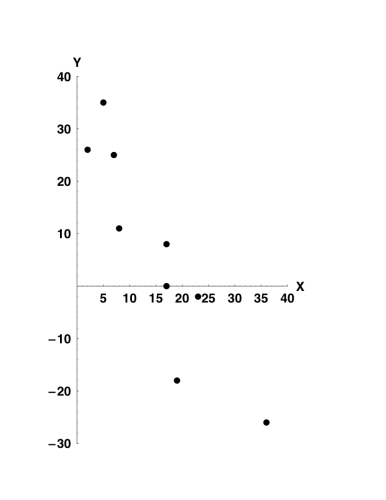
\includegraphics[scale=.5]{Foto/cr.png}
        \end{figure}
    \item La formula per calcolare il coefficiente di correlazione lineare è $$r_{xy}= \dfrac{s_{xy}}{\sqrt{s_{xx}s_{yy}}}$$. Calcolo allora $\overline{x}_9= 14.89$ e $\overline{y}_9= 6.56 $ e trovo $$r = \dfrac{-1576.44}{\sqrt{910.89 \cdot 3328.22}} = - 0.9$$ Troviamo quindi una forte correlazione lineare negativa.
    \item Trovo la retta di regressione di Y su X con la formula $y = \hat{\beta}x + \hat{\alpha}$. Trovo $\beta = \frac{S_{xy}}{S_{xx}} = \frac{-1576.44}{910.89} = -1.73$ e $\alpha = \overline{y} - \hat{\beta}\overline{x} = 6.56 - (-1.73) \cdot 14.89 = 32.32$ e trovo quindi la retta $$y=  -1.73x + 32.32$$
\end{itemize}

\ind \textbf{Soluzione punto 2}: Dal formulario è $ \left( \hat{\beta} \pm \sqrt{\dfrac{SS_R}{S_{xx}(n-2)}} t_{n-2, \sfrac{\alpha}{2}} \right)$ Conosco n=9, $\alpha/2 = 0.005$, $\hat{\beta}= -1.73$, $S_{xx} = 910.89$, mi manca trovare, attraverso formulario e tabelle $SS_R=599.94$ e $t_{7, 0.005}=3.499$ Dunque l'intervallo è $$-1.73 \pm \sqrt{\dfrac{599,94}{7 \cdot 910.89}} = (-2.80, -0.66)$$

\ind \textbf{Soluzione punto 3}: $H_0 :\beta = 0 \quad H_1 : \beta \neq 0$. Rifiutiamo l'ipotesi nulla se (dal formulario) $$\abs{\sqrt{\dfrac{S_{xx} (n-2)}{SS_R} \hat{\beta}} > t_{n-2, \sfrac{\alpha}{2}}}$$ Calcolo e trovo che $5.64 > 3.499$ e quindi rifiuto $H_0$. Questo test si poteva fare anche osservando l'IC in quanto $$\beta \notin(-2.80, -0.66) $$

\ind \textbf{Soluzione punto 4}: Per calcolare la bontà di adattamento del modello si utilizza il coefficiente di determinazione: $$R^2 = 1 - \frac{SS_R}{S_{yy}}= 1 - \frac{599.94}{3328.22} = 0.82$$ Questo significa che l'82\% della variazione delle risposte è giustificata dai predittori, quindi dal modello. Osservazione: dal coefficiente di determinazione ritroviamo il quadrato del coefficiente lineare, che possiamo trovare in modulo. Per il segno, sappiamo che il coefficiente lineare ha lo stesso segno di $\beta$ \n

\ind \textbf{Soluzione punto 5}: Per calcolare i residui posso calcolarli con la formula $ \overline{e_i} = y_i - \alpha -\beta x_i $. Trovo allora
\begin{figure}
    \centering
    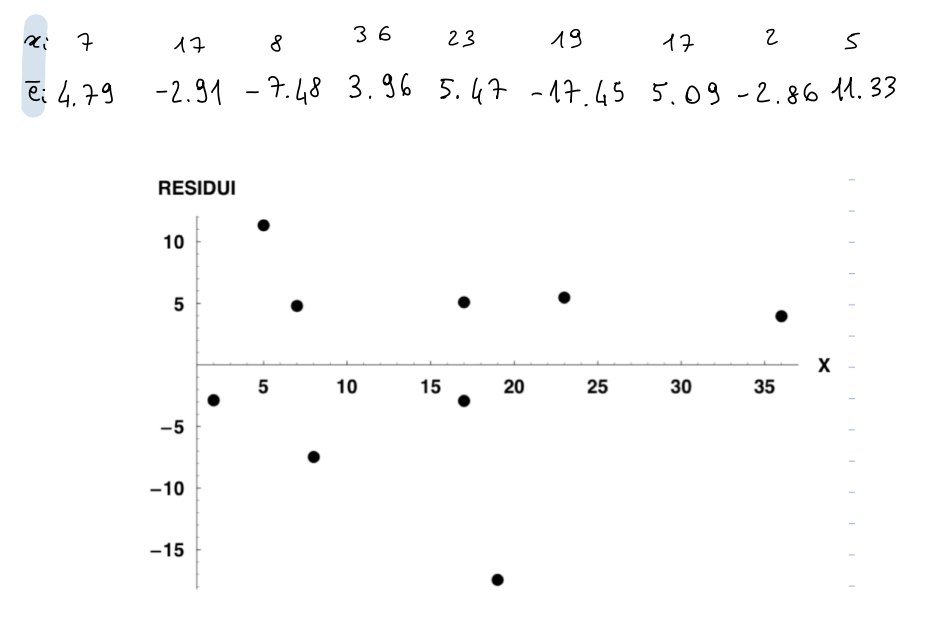
\includegraphics[scale=0.5]{Foto/c.png}
\end{figure}
I residui si dispongono in modo abbastanza casuale attorno all'asse x. 

\end{document}
